

\documentclass[../../tc_tp3_main.tex]{subfiles}

\begin{document}

\hyphenation{di-fe-ren-cial}
\hyphenation{cons-tan-te}
\hyphenation{ins-tru-men-ta-ción}
\hyphenation{pro-pues-ta}
%capítulo, Amplificadores de instrumentación
\chapter{Amplificadores de instrumentación}

%Introducción
\section{Introducción}

	%Notación
	A modo de delimitar un marco teórico y notacional a partir del cual se presentarán con mayor claridad y precisión los términos técnicos siguientes, se procede a definir las dos entradas genéricas, $V_1$ y $V_2$, de un circuito de tipo MISO (multiple inputs, single output) como: \par
	
	%Notación V_{CM} + V_{DMi}
 	\begin{equation}
  	   \left\{
	  	    \begin{array}{ll}
		 					\mathrm{V_1} = \mathrm{V_{CM} + V_{DM1}} \\
			 				\mathrm{V_2} = \mathrm{V_{CM} + V_{DM2}} \\
	     	 \end{array}
	     	\right.
 	\end{equation}
 	
	donde $V_{CM}$ es la tensión de modo común, es decir, la componente compartida por las dos señales $V_1$ y $V_2$, y $V_{DMi}$ es la tensión diferencial o la componente única/diferente de la tensión i, con i =1;2.\par
	Nótese que tanto $V_{CM}$ como $V_{DMi}$ pueden ser nulas o no, dependiendo de las señales $V_1$ y $V_2$ y de la relación existente entre ellas. \par
	En particular, cuando la señal $V_1$ y $V_2$ comparten el mismo canal de transmisión se podrá decir que las señales comparten el ruido proveniente del mismo\footnote{Sólo cuando la longitud de onda del ruido es muy superior al tamaño del circuito e interfieren con la medición} y por lo tanto $V_{CM}$ será una variable aleatoria de distribución de probabilidad acorde, a determinar. Además, aquellas señales que estén montadas sobre tensiones continuas también tendrán una componente continua común. \par
	Debe también hacerse notar el hecho de que $V_1 - V_2 = V_{DM1} - V_{DM2}$, por lo que el modo común se verá eliminado al restar las dos señales de input. De aquí se desprende la notación a utilizar para el modo diferencial: $V_{DM} = V_{DM1} - V_{DM2}$\par
	Esta notación permite expresar a las entradas del sistema MISO como un circuito dispuesto de la siguiente forma:\par 
	%circuito VCM y VDM
	\begin{center}
	\begin{circuitikz}[american voltages]
	\draw
	(6,0) to [short, *-] (3,0)
  to [V, l_=$\frac{V_{DM}}{2}$] (3,3) 
  (6,6) to [short, *-] (3,6)
  to [V, l^= $\frac{V_{DM}}{2}$] (3,3) 
  to [V, l^= $V_{CM}$] (0,3) 
	(0,3) to (0,1) node[ground]{}; 
  \end{circuitikz}
  \end{center}
  
	Una vez establecida la notación anterior, procedemos a definir los siguientes términos:\par
	
	%definición de términos técnicos- itemize
	\begin{itemize}
	
	%definición amplificador diferencial
	\item Un \underline{amplificador diferencial} es un circuito cuya función será atenúar significativamente el modo común (idealmente eliminarlo) de las dos entradas y amplificar el modo diferencial de las mismas, realizando la diferencia entre las dos señales.\par
	En efecto, teniendo en cuenta la linealidad del sistema o circuito, se puede tratar al efecto sobre las entradas por superposición, por lo que definiendo a la ganancia del modo común a la salida del circuito como $A_{CM}$ y a la del modo diferencial como $A_{DM}$, si H es el efecto del sistema sobre las entradas, entonces $H(V_{1};V_{2}) = A_{DM} * V_{DM} + A_{CM} * V_{CM}$\par
	
	A continuación se presenta un modelo típico de un amplificador de diferencias. 
	
	%circuito amp diferencial
	\begin{figure}[H]	
		\centering
		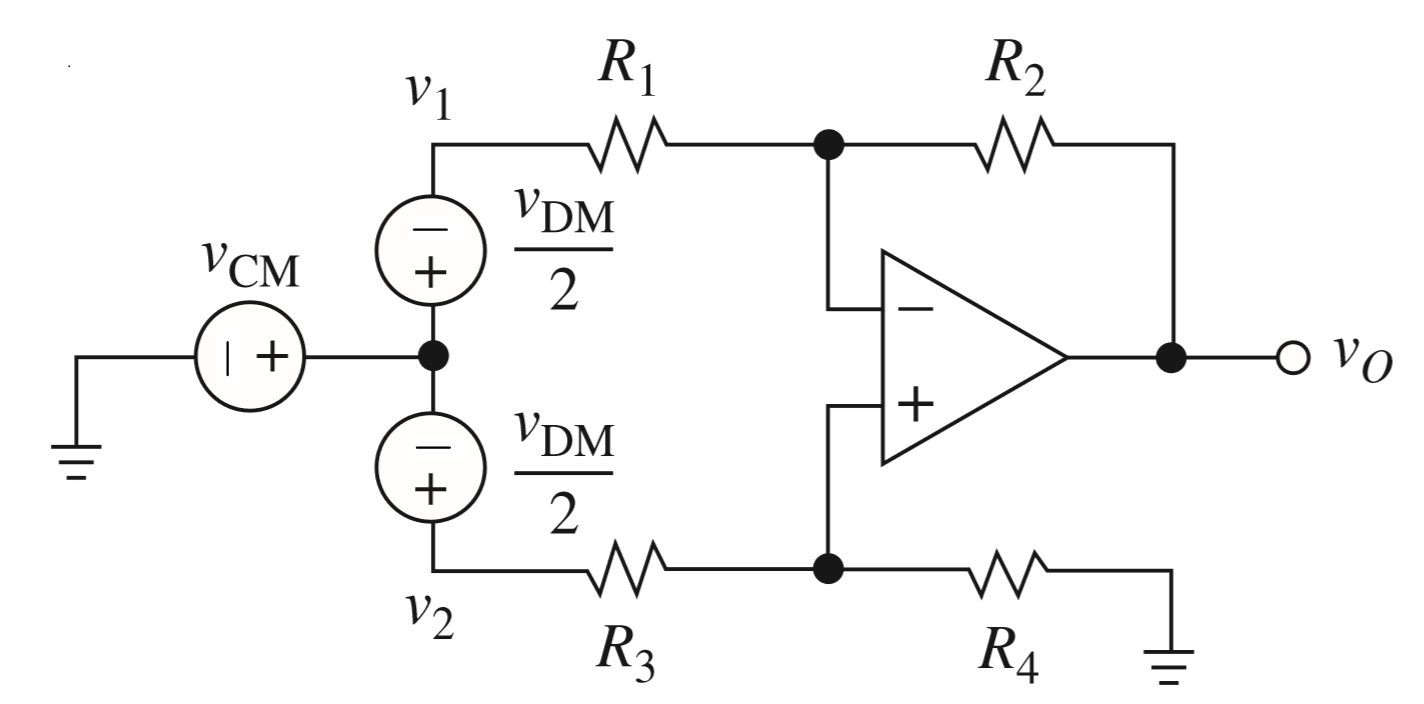
\includegraphics[scale=0.4]{imagenes/amp_diferencial.png}
		\caption{Modelo simple de amplificador diferencial}
		\label{fig:ej5_amp_diferencial}
	\end{figure}

	%definición CMRR
	\item El \underline{CMRR} o \underline{Common Mode Rejection Ratio} se define como la relación entre la ganancia del modo diferencial y el modo común, de forma tal que $CMRR =  \frac{A_{DM}}{A_{CM}}$. El mismo puede ser expresado en decibeles como $CMRR_{dB} =  20 \cdot \log_{10} {(\frac{A_{DM}}{A_{CM}})}$. \par
	La definición presentada anteriormente debe ser entendida entonces como una medida de cuánto prevalecerá el modo diferencial por sobre el modo común, es decir, permitirá cuantificar qué tan ''bueno'' es el amplificador diferencial: Cuanto mayor el CMRR, mejor cumple su función el amplificador diferencial. Así, un amplificador diferencial ideal tendrá un CMRR infinito. \par
	
	%definición amplificador de instrumentación
	\item Un \underline{amplificador de instrumentación} es un amplificador diferencial que cumple con las siguientes condiciones: \par
	
	\begin{enumerate}
		\item Impedancia de entrada muy grande (idealmente infinita) tanto para el modo diferencial como para el común.
		\item Impedancia de salida muy baja (idealmente nula).
		\item Ganancia estable y precisa.
		\item Un CMRR extremadamente grande.
	\end{enumerate}
	Cabe destacar que si un amplificador de instrumentación utilizara el modelo de amplificador diferencial presentado anteriormente, la impedancia de entrada del circuito sería finita y en consecuencia se cargaría el resto del circuito. Esto resultaría en un deterioro  de las señales de entrada, perdiéndose la tensión ideal que estas proveerían. Es así como se degradaría el CMRR, ya que el modo común conformado por el ruido no sufriría pérdida mientras la señal diferencial sí lo haría.\par
	Para solucionar este problema, se inserta un buffer en cada entrada, con una impedancia de entrada resultante infinita que idealmente no deterioraría la señal de entrada.\par
	
	En este trabajo se justificará el uso del diseño de un amplificador instrumental propuesto por la cátedra, al cual se le asignará valores específicos para los componentes, justificando también la elección de dichos valores y analizando su comportamiento, intentando corroborar la relación de lo teórico y simulado con lo práctico.\par

%termino definiciones- itemize	
	\end{itemize}
	
%presento el circuito
\section{Diseño del amplificador de instrumentación}

La cátedra propone un circuito con el cual se implementará un amplificador de instrumentación. Los valores de los componentes serán determinados mediante un análisis completo y detallado del circuito. 

%Diseño del circuito propuesto
	\begin{figure}[H]	
		\centering
		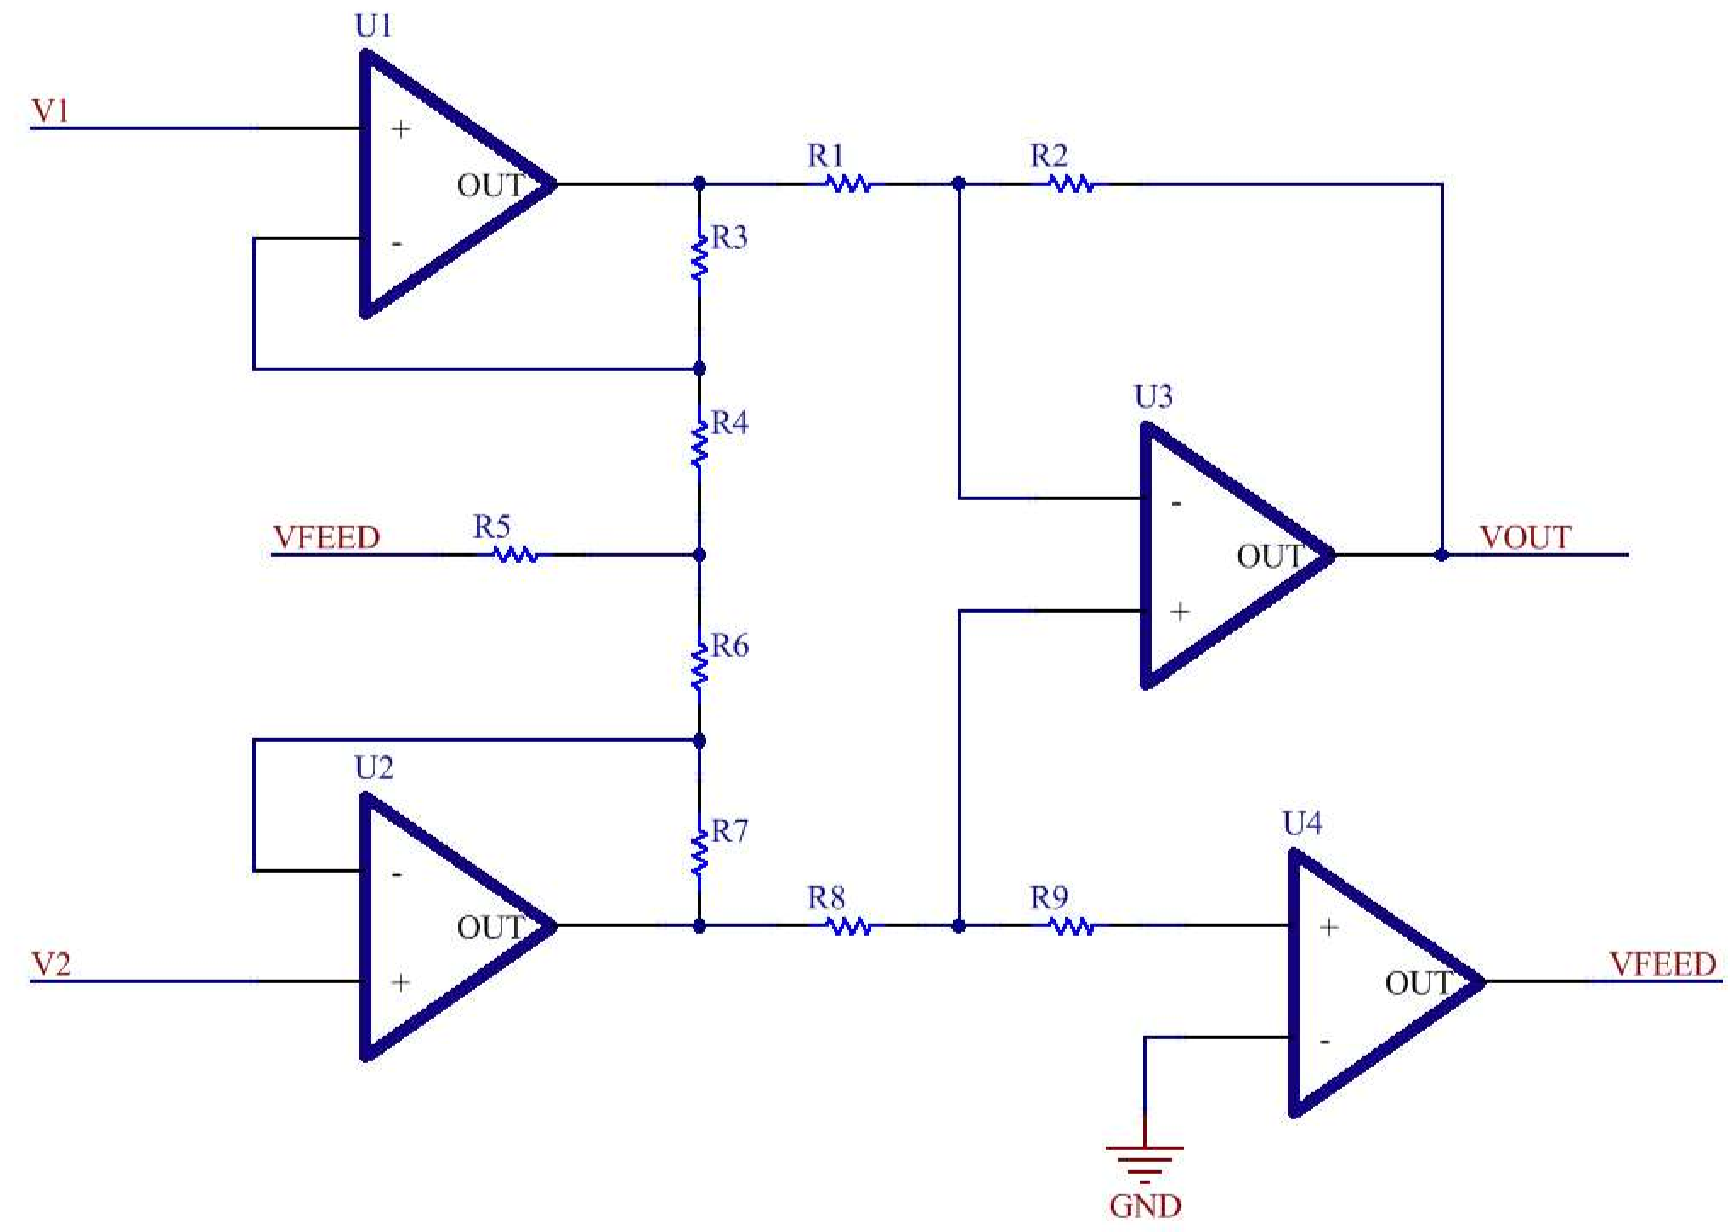
\includegraphics[scale=0.4]{imagenes/diseno_circuito.png}
		\caption{Circuito propuesto por la cátedra}
		\label{fig:ej3_diseno_circuito}
	\end{figure}
	
Al poseer 4 opamps, algunos con reatroalimentaciones entre sí, el tener en cuenta todas las no idealidades de estos 4 implicaría ecuaciones resultantes de alta complejidad y con tantas variables que el análisis sería engorroso y con pocas conclusiones que resulten de utilidad para los objetivos propuestos. Es por esto que las deducciones y los razonamientos con los cuales se podrá determinar los valores de los componentes para el buen funcionamiento del dispositivo provendrán de un análisis partido, con idealizaciones que se asuma contraerán un error bajo o aceptable y con algunos valores impuestos mediante la técnica de prueba y error a la hora de simular. \par
Primero, comenzaremos asumiendo que todos los opamps actúan bajo condiciones ideales.\par
	
%Análisis IDEAL del circuito
\subsection{Análisis ideal del circuito}

Para simplificar el análisis del circuito, como primer instancia se considera a todos los opamps ideales: cada uno con función transferencia constante para todas las frecuencias, impedancia de entrada infinita (y por lo tanto corrientes de entrada nulas)  y con tensiones iguales en las dos entradas.\par
Las condiciones mencionadas anteriormente reducen el circuito anterior a la siguiente figura: \par

%circuito ideal
	\begin{figure}[H]	
		\centering
		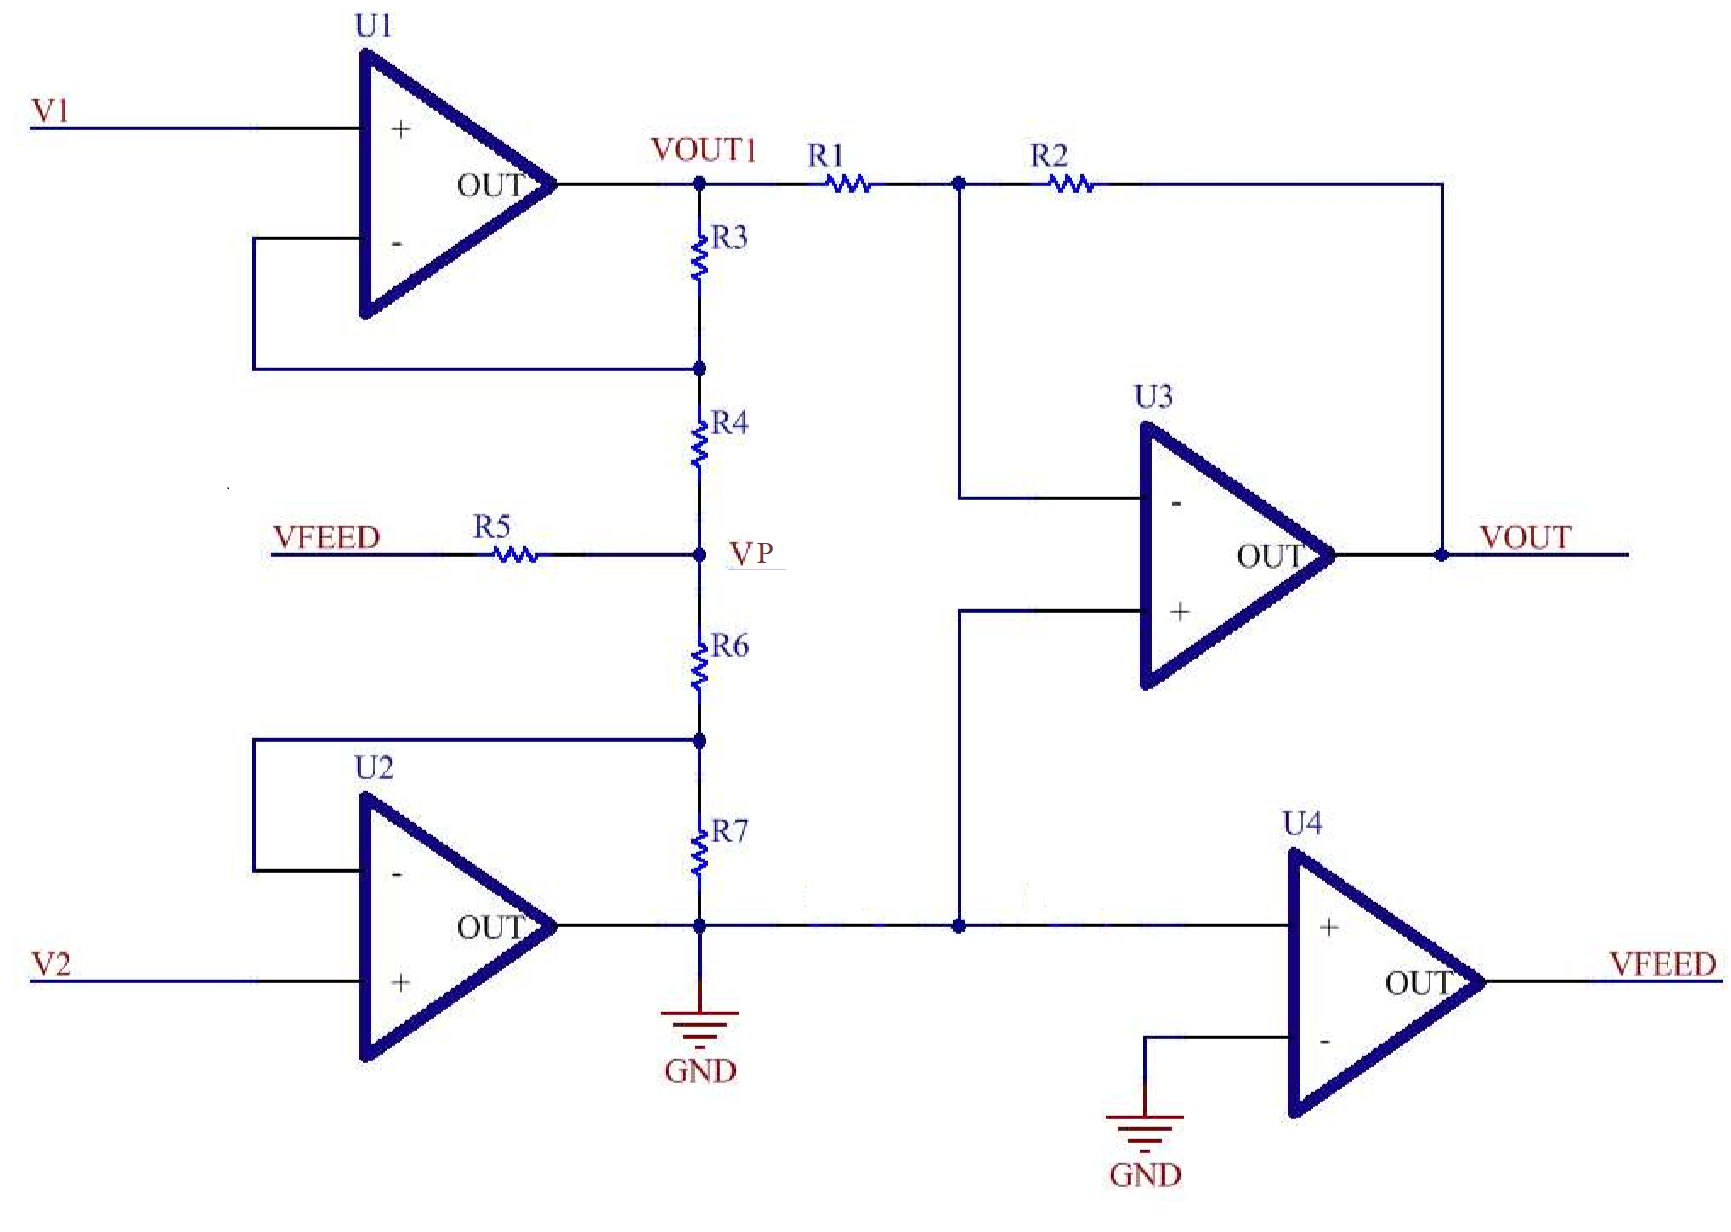
\includegraphics[scale=0.4]{imagenes/circuito_ideal.png}
		\caption{Circuito resultante con opamps ideales}
		\label{fig:ej3_circuito_ideal}
	\end{figure}
Por lo que, usando divisor resistivo, se plantea el siguiente sistema de ecuaciones: \par

%sistema de ecuaciones con opamp ideales
 	\begin{equation}
  	   \left\{
	  	    \begin{array}{ll}
		 					\mathrm{\frac{V_p}{R_4} - V_1\cdot (\frac{1}{R_4} + \frac{1}{R_3}) + \frac{V_{out1}}{R_3} = 0 } \\
			 				\mathrm{\frac{V_p}{R_6} - V_2\cdot (\frac{1}{R_6} + \frac{1}{R_7}) = 0 } \\
			 				\mathrm{\frac{V_{out1}}{R_1} + \frac{V_{out}}{R_2} = 0 } \\
	     	 \end{array}
	     	\right.
 	\end{equation}
 	
del cual se puede calcular la señal de salida en función de las entradas como: \par

$V_{out} = \frac{R_2\cdot [R_3\cdot (R_6 + R_7) \cdot V_2 -R_7\cdot (R_4 + R_3)\cdot V_1]}{R_1\cdot R_4\cdot R_7}$

Dado que se requiere que la salida sea directamente proporcional a la resta de las dos señales, para eliminar el modo común, se pide que:\par
\begin{centering}
$R_3\cdot (R_6 + R_7) = R_7\cdot (R_4 + R_3)$\par
\end{centering}
que resulta en la condición: \par
\begin{centering}
$\frac{R_3}{R_4} = \frac{R_7}{R_6}$\par
\end{centering}
Y cuya función transferencia final es: \par
$V_{out} = \frac{R_2\cdot R_7\cdot (R_4 + R_3)}{R_1\cdot R_4 \cdot R_7}\cdot (V_1 - V_2)$\par
Entonces: \par

%funcion transferencia ideal
\fbox{
				\centering
       $V_{out} = \frac{R_2}{R_1}\cdot (1 + \frac{R_3}{R_4})\cdot (V_1 - V_2)$
}

Esta relación ideal muestra una ganancia en modo diferencial potencialmente grande y constante para todas las frecuencias. De esta manera el modelo ideal cumple efectivamente con el modelo de un amplificador de instrumentación. Además, se logra un CMRR ideal infinito, es decir que el modo común sería eliminado en su totalidad en un análisis ideal. \par
Tanto por comodidad como para lograr simetría en la primera etapa de amplificación (como se explicará más adelante), se tomo $R_3 = R_7$ y $R_4 = R_6$
Luego, en el contexto ideal, si se requiere una ganancia $X$, se puede solucionar este problema mediante las siguientes asignaciones: \par
 	\begin{equation}
  	   \left\{
	  	    \begin{array}{ll}
		 					\mathrm{\sqrt{X} = \frac{R_2}{R_1} } \\
			 				\mathrm{\sqrt{X} - 1 = \frac{R_3}{R_4}} \\
	     	 \end{array}
	     	\right.
 	\end{equation}
 	por lo que la razón $\frac{R_7}{R_6}$ quedaría también determinada como $\frac{R_7}{R_6} = \sqrt{X} - 1$ por la relación antes propuesta. Nótese que esta asignación busca una ganancia repartida de manera equitativa o uniforme entre las dos estapas de amplificación, una dada por la relación $\frac{R_3}{R_4}$ y otra por $\frac{R_2}{R_1}$\par
 	Sin embargo, según la fórmula de Friis, cuando se conecta opamps en cascada la ganancia deberá ser superior en las últimas etapas de amplificación (en nuestro caso en $1+\frac{R_3}{R_4}$) para disminuir la amplificación del ruido. Es por esto que se decidió hacer que la ganancia fuera superior en la segunda etapa. Esta decisión, como se comentará más adelante, fue errónea: el opamp U4 tiene realimenta a los opamps U1 y U2, por lo que este sistema resulta ser circular y por ende la fórmula no tiene el sentido que antes tenía. Se cree que es por esta razón el sistema osciló en un primer intento de confección, contrario a lo que mostraban las simulaciones.\par
El problema se solucionó al alterar los valores de las resistencias para que la ganancia fuese más balanceada y aumentando el valor de $R_5$, que según mostraron las simulaciones y la función de transferencia no ideal (más en detalle más adelante), tenía una gran influencia sobre la estabilidad del circuito, al determinar dónde se encuentran los polos de esta función.\par
 	
 	Interpretando el análisis anterior, se puede decir que el sistema idealmente busca la simetría en la primera etapa de modo tal que las corrientes del medio para las resistencias $R_4, R_3$ y $R_6, R_7$ sean nulas. Esto implicaría que el modo común pasaría inadvertido por la primera etapa, procediendo a ser eliminado por el opamp restador de la segunda etapa. Su fundamento es el teorema de simetría: Si un circuito puede ser descompuesto en dos emi circuitos iguales de forma tal que el circuito pueda ser expresado como la conexión simétrica de estos emi circuitos mediante cables, y si las tensiones de entrada están cada una conectada a un emi circuito, entonces si las tensiones de entrada son iguales entre sí, las corrientes de los cables conectores serán nulas. Es aquí donde planteamos el problema de las tolerancias de las resistencias y con ello la razón de ser del opamp U4.
 	
\subsection{Análisis de tolerancias para el caso ideal}

Se intenta buscar el efecto de las tolerancias sobre la ganancia ideal del circuito.\par
Se hace notar que si una resistencia real $R$ tuviera una variación sobre su valor ideal de $\Delta x$, entonces ya no se cumpliría la condición $R_3\cdot (R_6 + R_7) = R_7\cdot (R_4 + R_3)$ mencionada en el tratamiento ideal, por lo que el modo común no se vería totalmente eliminado como se planeaba.\par 
Es aquí donde entra en juego el funcionamiento del opamp U4, que viene a realizar la calibración del circuito, reacomodando la tensión del punto medio Vp mediante VFEED y $R_5$ para que en este punto haya una tensión de 0V o lo más cercana posible a este valor cosa tal de que se siga cumpliendo la simetría necesaria para eliminar al modo común. 
Este opamp intentará forzar la tierra virtual sobre la entrada negativa, teniendo para esto que acomodar su tensión de salida de forma acorde. \par
Si la tensión de entrada del cuarto opamp no fuera nula, se lograría por lo tanto una tensión de offset, ya que se intentaría forzar en el punto medio la tensión anterior más un corrimiento dado por el cambio de tensión de la tierra virtual. \par
Un análisis más comprensivo de lo dicho anteriormente es siguiendo el razonamiento de las corrientes mencionadas anteriormente: En caso de no cumplirse la simetría deseada, las corrientes intermedias dejarán de ser nulas y por ende forzarán caídas de tensión distintas en cada extremo. Las distintas corrientes causarán un desbalance a la entrada de los opamps: El opamp U4 tendrá que suplir entonces con una corriente a su salida tal que el anterior equilibro se logre de nuevo y las corrientes intermedias vuelvan a ser nulas, para que se produzca la resta y con esto se elimine el modo común.\par
 Como la caída sobre la resistencia R9 cambiará con la corriente de entrada del opamp U4, con la corriente de entrada se cambiará la tensión de la tierra virtual, que deberá ser acomodada por el opamp con una tensión y corriente de salida correspondiente.\par
 Es así como se logra la calibración en tiempo continuo del circuito mediante la presencia del opamp U4.\par

  
%Análisis no ideal
\subsection{Análisis \underline{NO} ideal del circuito}

Se puede obtener la transferencia total del circuito en modo diferencial y en modo común por separado teniendo en cuenta las limitaciones propias de los opamps que conforman el circuito. Estas limitaciones están dadas por la consideración de una ganancia y una impedancia de entrada finitas (aunque muy grandes) y una respuesta en frecuencia con polo dominante.\par
Sin embargo, la función transferencia del circuito utilizando estos modelos resulta tener una complejidad demasiado grande para realizar un análisis exhaustivo que resulte provechoso contra un análisis realizado por prueba y error mediante simulaciones con estas propiedades para cada opamp en LTSPICE. Sin embargo, dicho análisis teórico se ha hecho porque así lo pedía la consigna del trabajo. Se consideró la respuesta en frecuencia de todos los opamps con polo dominante e impedancia de entrada finita para todos menos el opamp U4. Al final de esta subsección se muestra tanto el sistema de ecuaciones como el despeje básico mediante el cual se intentó reducir la expresión a algo manejable, sin éxito.\par
Por la complejidad de la función de transferencia, se decidió utilizar las relaciones de resistencias antes mencionados en la consideración ideal y luego determinar valores apropiados para R5, R8 y R9 mediante iteraciones inteligentes en LTSPICE, observando tanto la respuesta en frecuencia como la transitoria para verificar que se pudiese obtener la ganancia requerida y estabilidad en el sistema.\par
Estas simulaciones arrojaron rangos de valores para R8 y R9 para que la ganancia ideal con el planteo anterior no se viese alterada significativamente y de R5 para lograr que el circuito convergiese a la ganancia esperada y no oscilara (sea inestable) ni atenuara toda la señal en su totalidad, ni tampoco amplificara tanto el modo común y el modo diferencial a la vez.  Dentro de los rangos mencionados, se eligió un valor intermedio para que los posibles desvíos de los valores reales originados por las tolerancias (1\%para SMD, que fue lo que se decidió utilizar) no interfirieran en la ganancia ideal.\par
Cabe destacar a su vez que variaciones en el valor de R5 alteraban enormemente al valor de VFEED, por lo que se requirió un análisis más detallado de la función del cuarto opamp y de R5 para lograr entender al circuito en mayor profundidad y así poder encontrar los valores apropiado. Este análisis fue presentado en la subsección anterior. Es importante señalar también que variaciones en R8 y R9 no modifican significativamente la ganancia ideal, pero que se buscó optimizar este valor ideal con los valores elegidos por simulación.\par
 
 Para el análisis analítico, se planteó el siguiente sistema de ecuaciones en Matlab: 
 
 \lstset{language=Matlab,%
    %basicstyle=\color{red},
    breaklines=true,%
    morekeywords={matlab2tikz},
    keywordstyle=\color{blue},%
    morekeywords=[2]{1}, keywordstyle=[2]{\color{black}},
    identifierstyle=\color{black},%
    stringstyle=\color{mylilas},
    commentstyle=\color{mygreen},%
    showstringspaces=false,%without this there will be a symbol in the places where there is a space
    numbers=left,%
    numberstyle={\tiny \color{black}},% size of the numbers
    numbersep=9pt, % this defines how far the numbers are from the text
    emph=[1]{for,end,break},emphstyle=[1]\color{red}, %some words to emphasise
    %emph=[2]{word1,word2}, emphstyle=[2]{style},    
}


\section*{Matlab Code}

\lstinputlisting{trans_no_ideal.m}

que conlleva una expresión de 6500 caracteres, que a su vez puede simplificarse aún más tratando al numerador y al denominador por separado, con los coeficientes de cada potencia de $s$ también por separado. Se usó el código de java del anexo para poder parsear con simplificidad la función de transferencia. Esta terminó con una forma del estilo $V_{out} = (V_1 - V_2)\cdot H(s)$ solamente en el caso en que $R_1 = 0$, lo cual no coincide con el análisis ideal. Se muestra en el anexo la función de transferencia simplificada para el caso en que $R_1$ = 0.\footnote{La versión impresa en la que $R_1$ no es nula será presentada en el examen oral si así se requiere} Independientemente de si $R_1$ fuera nula o no, la transferencia H(s) tendría la forma $\frac{N(s)}{D(s)}$, donde N(s) es un polinomio de orden 2 de s y D(s) un polinomio de orden 4 de s. Dado la complejidad del análisis de ceros para un polinomio de orden 4 y la extensión de su expresión, un análisis de polos para H(s) resulta completamente impráctica para resolver problemas de estabilidad y de ganancia constante y precisa, condiciones necesarias para todo amplificador de instrumentación. Es por esto que se recurrió a la simulación. \par
Se llega entonces a la conclusión de que si los polos de la H(s) estuviesen todos del lado izquierdo del eje imaginario (la parte real de los polos fuese negativa) y la función fase de H(s) no llegase a los 180\textdegree dentro de un margen seguro, entonces se podría asegurar que el circuito será estable. Un análisis más detallado en estos términos resulta también impráctico con los conocimientos actuales (todavía no se ha visto en profundidad el criterio de Barkhausen ni métodos para identificar lazos de retroalimentación) .\par

Mediante simulaciones, se determinó que los valores de R5 para garantizar la convergencia debían ser superiores o iguales a 10k\ohm, y se simuló con valores hasta 50k\ohm.\par
Por otra parte, se eligió por comodidad que los valores de $R_8$ y $R_9$ fueran iguales. Se observó que valores de entre 100\ohm y 5K\ohm garantizaban estabilidad para los valores mencionados anteriormente de $R_5$ y la ganancia teórica ideal del análisis anterior.\par


%implementación, fijamos valores
\subsection{Implementación del circuito}

Se busca implementar un amplificador de instrumentación con una ganancia en modo diferencial $G$ dada por 
$G = 120 + 20\cdot sen(\frac{3\cdot\pi}{4}+\frac{\pi}{6}) \approx 125.17$\par

El primer intento de confección del circuito (el cual osciló, originando una salida senoidal montada a otra senoidal), intentó discriminar entre etapas de ganancia, otorgando una ganancia mucho mayor a la primer etapa de amplificación. Al intentar solucionar la oscilación, se decidió modificar los valores de los componentes elegidos. Se cometió un error al hacer esta substitución en el cálculo de los valores para la ganancia ideal. Es por esta razón que con los valores elegidos se obtuvo una ganancia del orden de las 136 veces para el modo diferencial en vez de las 125 esperadas. \par

Los valores finales para las resistencias elegidas fueron:\par

\begin{enumerate}
	\item $R_3 = R_7 = 15k\ohm$
	\item $R_4 = R_6 = 1.3k\ohm$
	\item $R_8 = R_9 = 1k\ohm$
	\item $R_2 = 68k\ohm$
	\item $R_1 = 6.2k\ohm$
	\item $R_5 = 20k\ohm$ 
\end{enumerate}

Se eligieron valores del orden de los 10 k\ohm porque impedancias de alto valor se corresponden con altos valores de ruido ya que variaciones muy pequeñas de corriente debido a la presencia de ruido producirán grandes cambios de tensión, aumentando así el ruido del sistema. Es por esto que se evitó agregar ruido extra al sistema al no utilizar impedancias altas.\par
El integrado utilizado en el primer intento fue un TL084, pero debido a que el mismo dejo de funcionar y a que en el pañol no se contaba con otro TL084, se utilizó el TL074, que luego se supo tenía mayor tolerancia al ruido, lo cual benefició al circuito.


%Puente de Wheatstone
\section{Diseño de un generador de señales de baja amplitud}
Se pretende desarrollar un generador de señales de baja amplitud mediante el uso de un \underline{puente de wheatstone}, que cumple con el siguiente modelo:

%circuito puente
	\begin{figure}[H]	
		\centering
		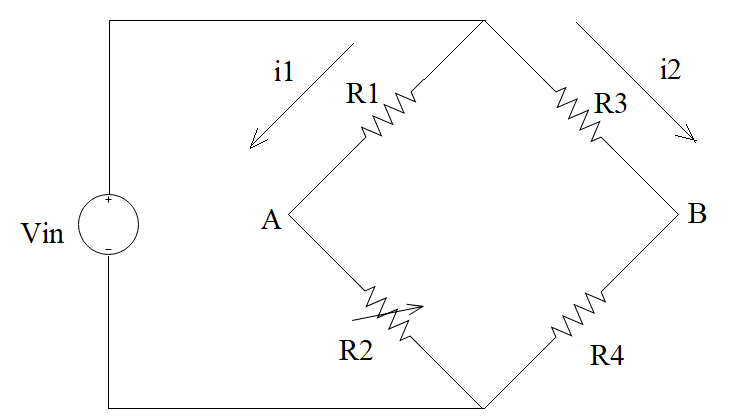
\includegraphics[scale=0.8]{imagenes/puente_wheatstone.png}
		\caption{Modelo del puente de wheatstone}
		\label{fig:ej5_puente_wheatstone}
	\end{figure}

Del cual se pueden obtener las siguientes ecuaciones: 

%sistema de ecuaciones para el puente
 	\begin{equation}
  	   \left\{
	  	    \begin{array}{ll}
		 					\mathrm{V_{in} = i_1\cdot (R_1 + R_2) } \\
			 				\mathrm{V_{in} = i_2\cdot (R_3 + R_4) } \\
		 					\mathrm{V_{a} = i_1\cdot R_1 } \\
			 				\mathrm{V_{b} = i_2\cdot R_3 } \\
	     	 \end{array}
	     	\right.
 	\end{equation}

De donde se puede obtener que $V_{a} - V_{b} = V_{ab} = V_{in} \cdot (\frac{R_1}{R_2} - \frac{R_3}{R_4})$
Además, de aquí se observa que si se toma los valores de las resistencias fijas y de la variable de forma tal que $\frac{R_3}{R_4} = \frac{R_1}{R_2}$ resulta que  $V_{ab} = 0$. \par
Es así como, tomando la salida del circuito sobre $V_{ab} = V_{out}$ se puede lograr una salida nula, y haciendo variar a $R_2$ se logrará variar también la tensión de salida, siendo ésta inversamente proporcional al cambio sobre $R_2$. Así, con pequeñas variaciones sobre $R_2$ se podrá lograr una salida de amplitud muy baja. \par

%Análisis de tolerancias
\subsection{Análisis de tolerancias}
Las resistencias a utilizar tendrán las mismas tolerancias. Se eligió utilizar resistencias SMD por su menor tolerancia, del 1\%. \par
Si $\Delta x_i$ es el error del valor nominal de la resistencia $R_i$ versus su valor real y si $E_{R_i}$ es el error total (en valor absoluto) que tiene ese error sobre la tensión de salida real con respecto a la teórica, entonces se obtiene:

%Error de tolerancias!
 	\begin{equation}
  	   \left\{
	  	    \begin{array}{ll}
		 					\mathrm{\frac{\partial V_{out}}{\partial R_1} = \frac{V_{in}}{R_2}} \\
			 				\mathrm{\frac{\partial V_{out}}{\partial R_2} = -\frac{V_{in} \cdot R_1}{R_2^2} } \\
	     	 \end{array}
	     	\right.
 	\end{equation}
por lo que 

 	\begin{equation}
  	   \left\{
	  	    \begin{array}{ll}
		 					\mathrm{E_{R_1} = \int_{R1 - \Delta x_1}^{R1 + \Delta x_1} {\frac{V_{in}}{R_2} dR_1}  }\\
			 				\mathrm{E_{R_2} =  \int_{R2 - \Delta x_2}^{R2 + \Delta x_2} -\frac{V_{in} \cdot R_1}{R_2^2} dR_2 }  \\
	     	 \end{array}
	     	\right.
 	\end{equation}
y de aquí que:
 	\begin{equation}
  	   \left\{
	  	    \begin{array}{ll}
		 					\mathrm{E_{R_1} = \frac{V_{in}}{R_2} \cdot 2\cdot \Delta x_1}\\
			 				\mathrm{E_{R_2} =  V_{in} \cdot R_1\cdot \frac{2\cdot \Delta x_2}{R_2^2-\Delta x_2^2}}  \\
	     	 \end{array}
	     	\right.
 	\end{equation}
 	
 	Si se toma en cuenta que la tolerancia es del 1\%, entonces $\Delta x_i = R_i \cdot 0.01$, y utilizando estos resultados:
 	
 	 	\begin{equation}
  	   \left\{
	  	    \begin{array}{ll}
		 					\mathrm{E_{R_1} = \frac{V_{in}}{R_2} \cdot 2\cdot 0.01 \cdot R_1 = 0.02 \cdot \frac{V_{in}\cdot R_1}{R_2}}\\
			 				\mathrm{E_{R_2} =  \frac{V_{in} \cdot R_1}{R_2}\cdot \frac{0.02}{1-0.01^2} \approx 0.02 \cdot \frac{V_{in} \cdot R_1}{R_2}}  \\
	     	 \end{array}
	     	\right.
 	\end{equation}
Los errores $E_{R_3}$ y $E_{R_4}$ son obtenidos análogamente, por lo que resulta que :

 	 	 	\begin{equation}
  	   \left\{
	  	    \begin{array}{ll}
		 					\mathrm{E_{R_3} = 0.02 \cdot \frac{V_{in}\cdot R_3}{R_4}}\\
			 				\mathrm{E_{R_4}  \approx 0.02 \cdot \frac{V_{in} \cdot R_3}{R_4}}  \\
	     	 \end{array}
	     	\right.
 	\end{equation}
 	El error total máximo será por lo tanto $E = E_{R_1} + E_{R_2} + E_{R_3} + E_{R_4}$\par
 	Dado que el puente mencionado será utilizado para generar tensiones de baja amplitud, en valores de tensión de salida cercanos a cero $\frac{R_1}{R_2}\approx\frac{R_3}{R_4}$, por lo que $E_{R_1} \approx E_{R_2} \approx E_{R_3} \approx E_{R_4}$. De esta forma: \par
 	$E \approx 0.08 \cdot \frac{V_{in}\cdot R_3}{R_4}$. De aquí se observa que si el cociente teórico $\frac{R_3}{R_4}$ se mantiene bajo, entonces el error también lo será para amplitudes bajas de tensión se salida. Una tensión $V_{in}$ apropiadamente elegida también implicará un menor error.\par
 	Una posible solución a este problema sería medir las resistencias fijas antes de colocarlas en el puente, de manera tal de conocer el valor exacto del cociente $\frac{R_3}{R_4}$ y el valor de $R_1$. Así, se podría luego determinar fácilmente el valor de $R_2$ que logrará tensión nula y de allí determinar el rango de valores que deberá tomar la $R_2$ para el rango de tensiones que se querrá tomar como salida. \par
 	Otra manera de solucionar el problema de tolerancias sería agregar presets en serie con las resistencias, para acomodar los valores reales a los valores teóricos previamente calculados.\par
 	Debe hacerse notar que del problema de las tolerancias se desprenden dos errores importantes: En el caso en que se desconociesen los valores reales de las resistencias antes o después de haberlas insertado en el circuito, no habría forma de determinar que valor de resistencia del preset haría que la salida sea nula completamente, por lo que se tendría que medir la salida en tiempo real para ubicar este punto. \par
 	El segundo problema es que el nuevo generador de señales será asimetrico en amplitud:
 	
%Tierra compartida
\subsection{Importancia de la tierra compartida para generar señales}

El generador con la salida del amplificador de instrumentación deberán compartir tierra, es decir, deberán ser conectados de la siguiente manera:

%disposición de tierra compartida con amp
	\begin{figure}[H]	
		\centering
		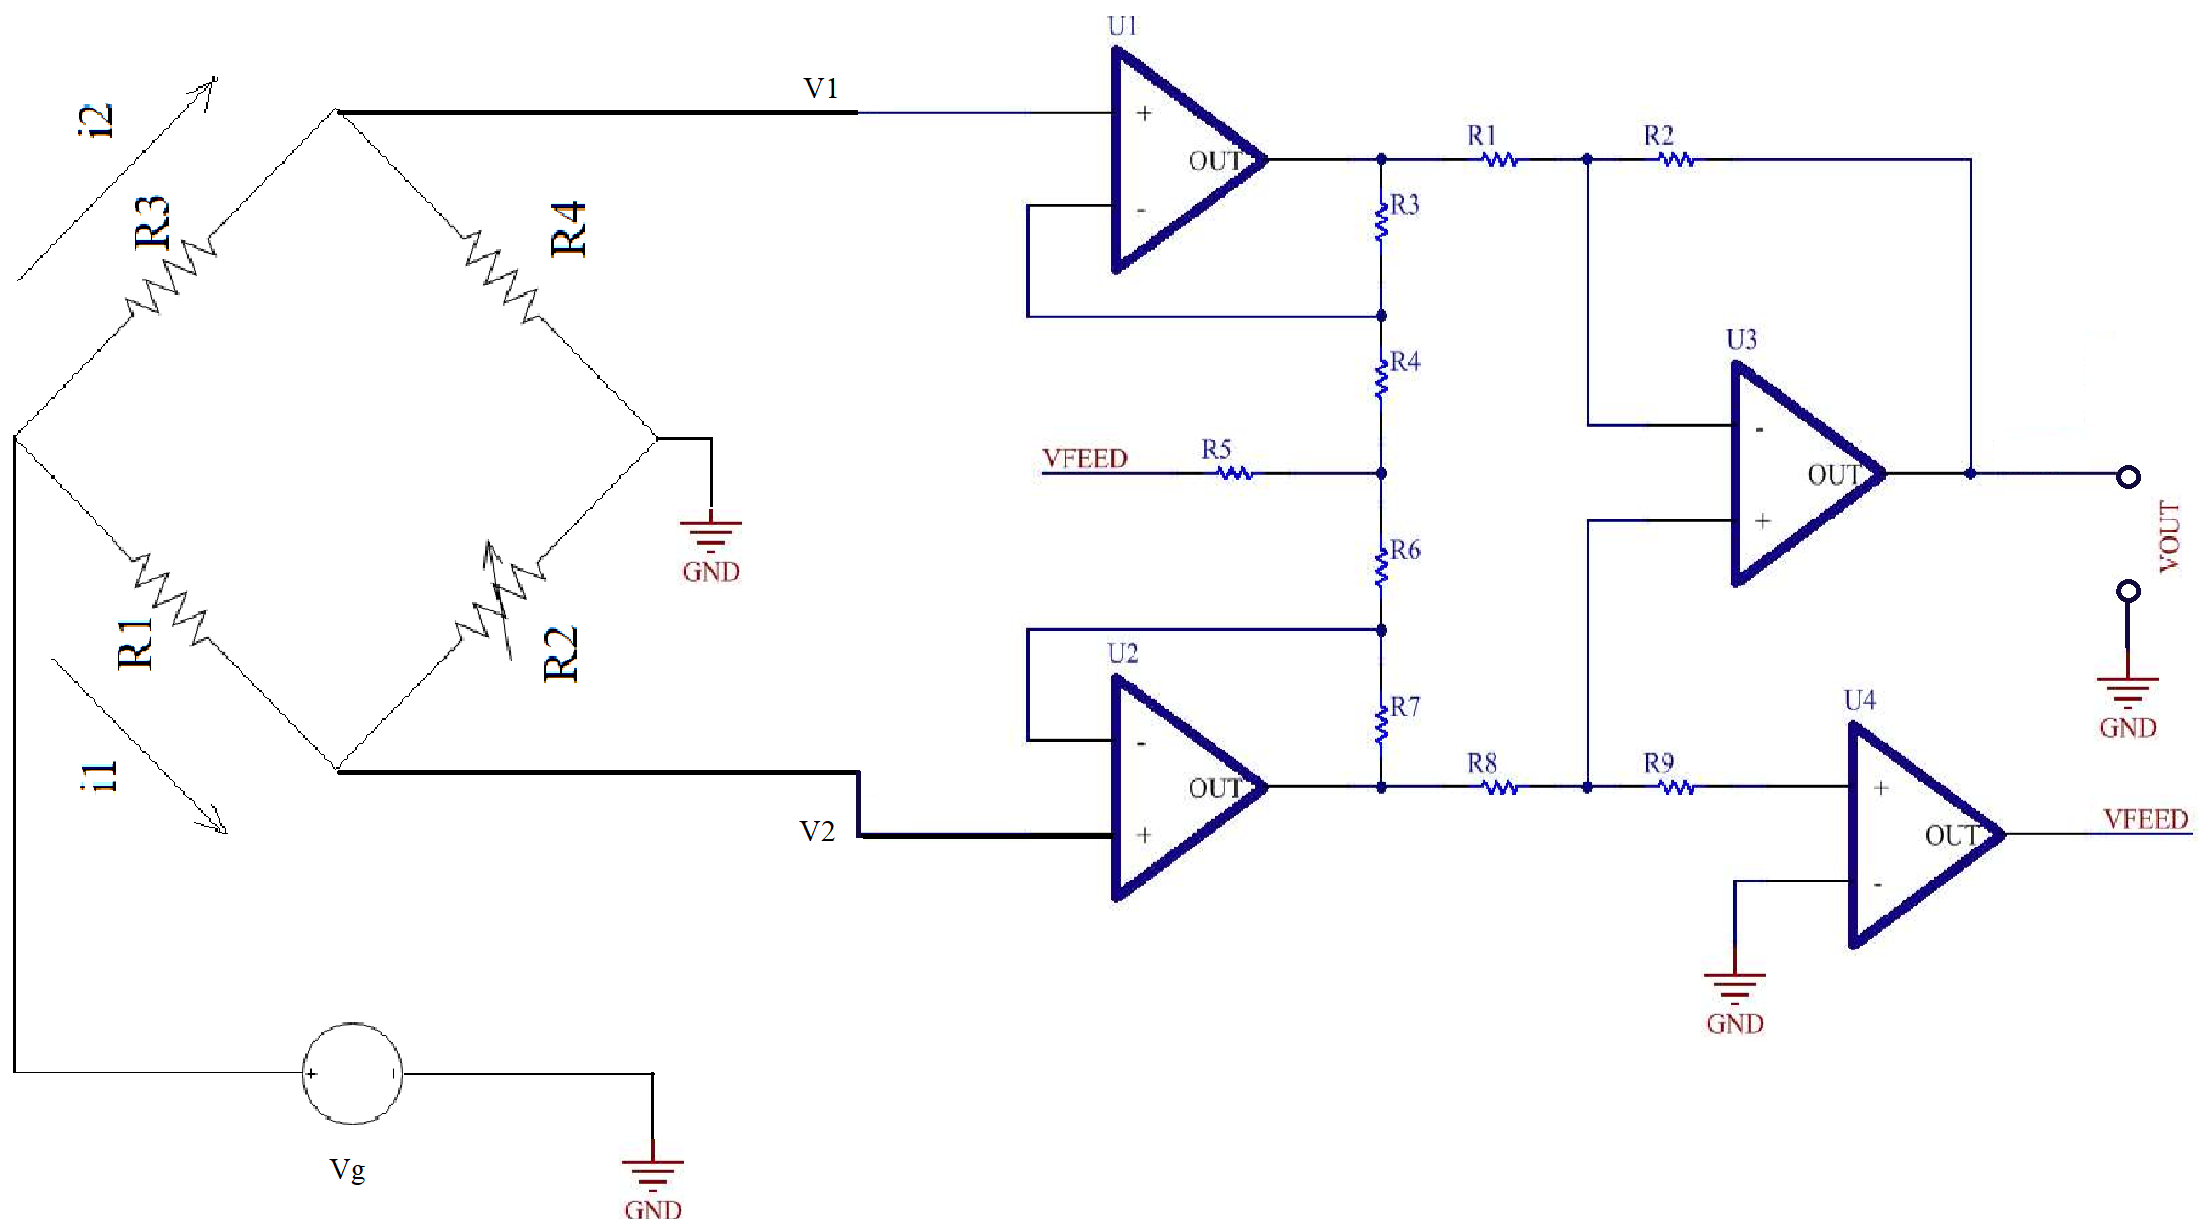
\includegraphics[scale=0.3]{imagenes/tierra_amp.png}
		\caption{Disposición del circuito con generador, tierra compartida.}
		\label{fig:ej5_tierra_amp}
	\end{figure}

Esto es así porque en el caso en que la salida no comparta tierra con el generador (como en la siguiente figura), el amplificador de instrumentación eliminará al modo común, y con éste al error, proveniente de la tierra del generador pero a la salida se le sumará un nuevo error proveniente de la segunda tierra, la de la salida. Es así como en el caso en que no se comparta la tierra el amplificador de instrumentación deja de funcionar correctamente.\par

%disposición de tierra NO compartida con amp
	\begin{figure}[H]	
		\centering
		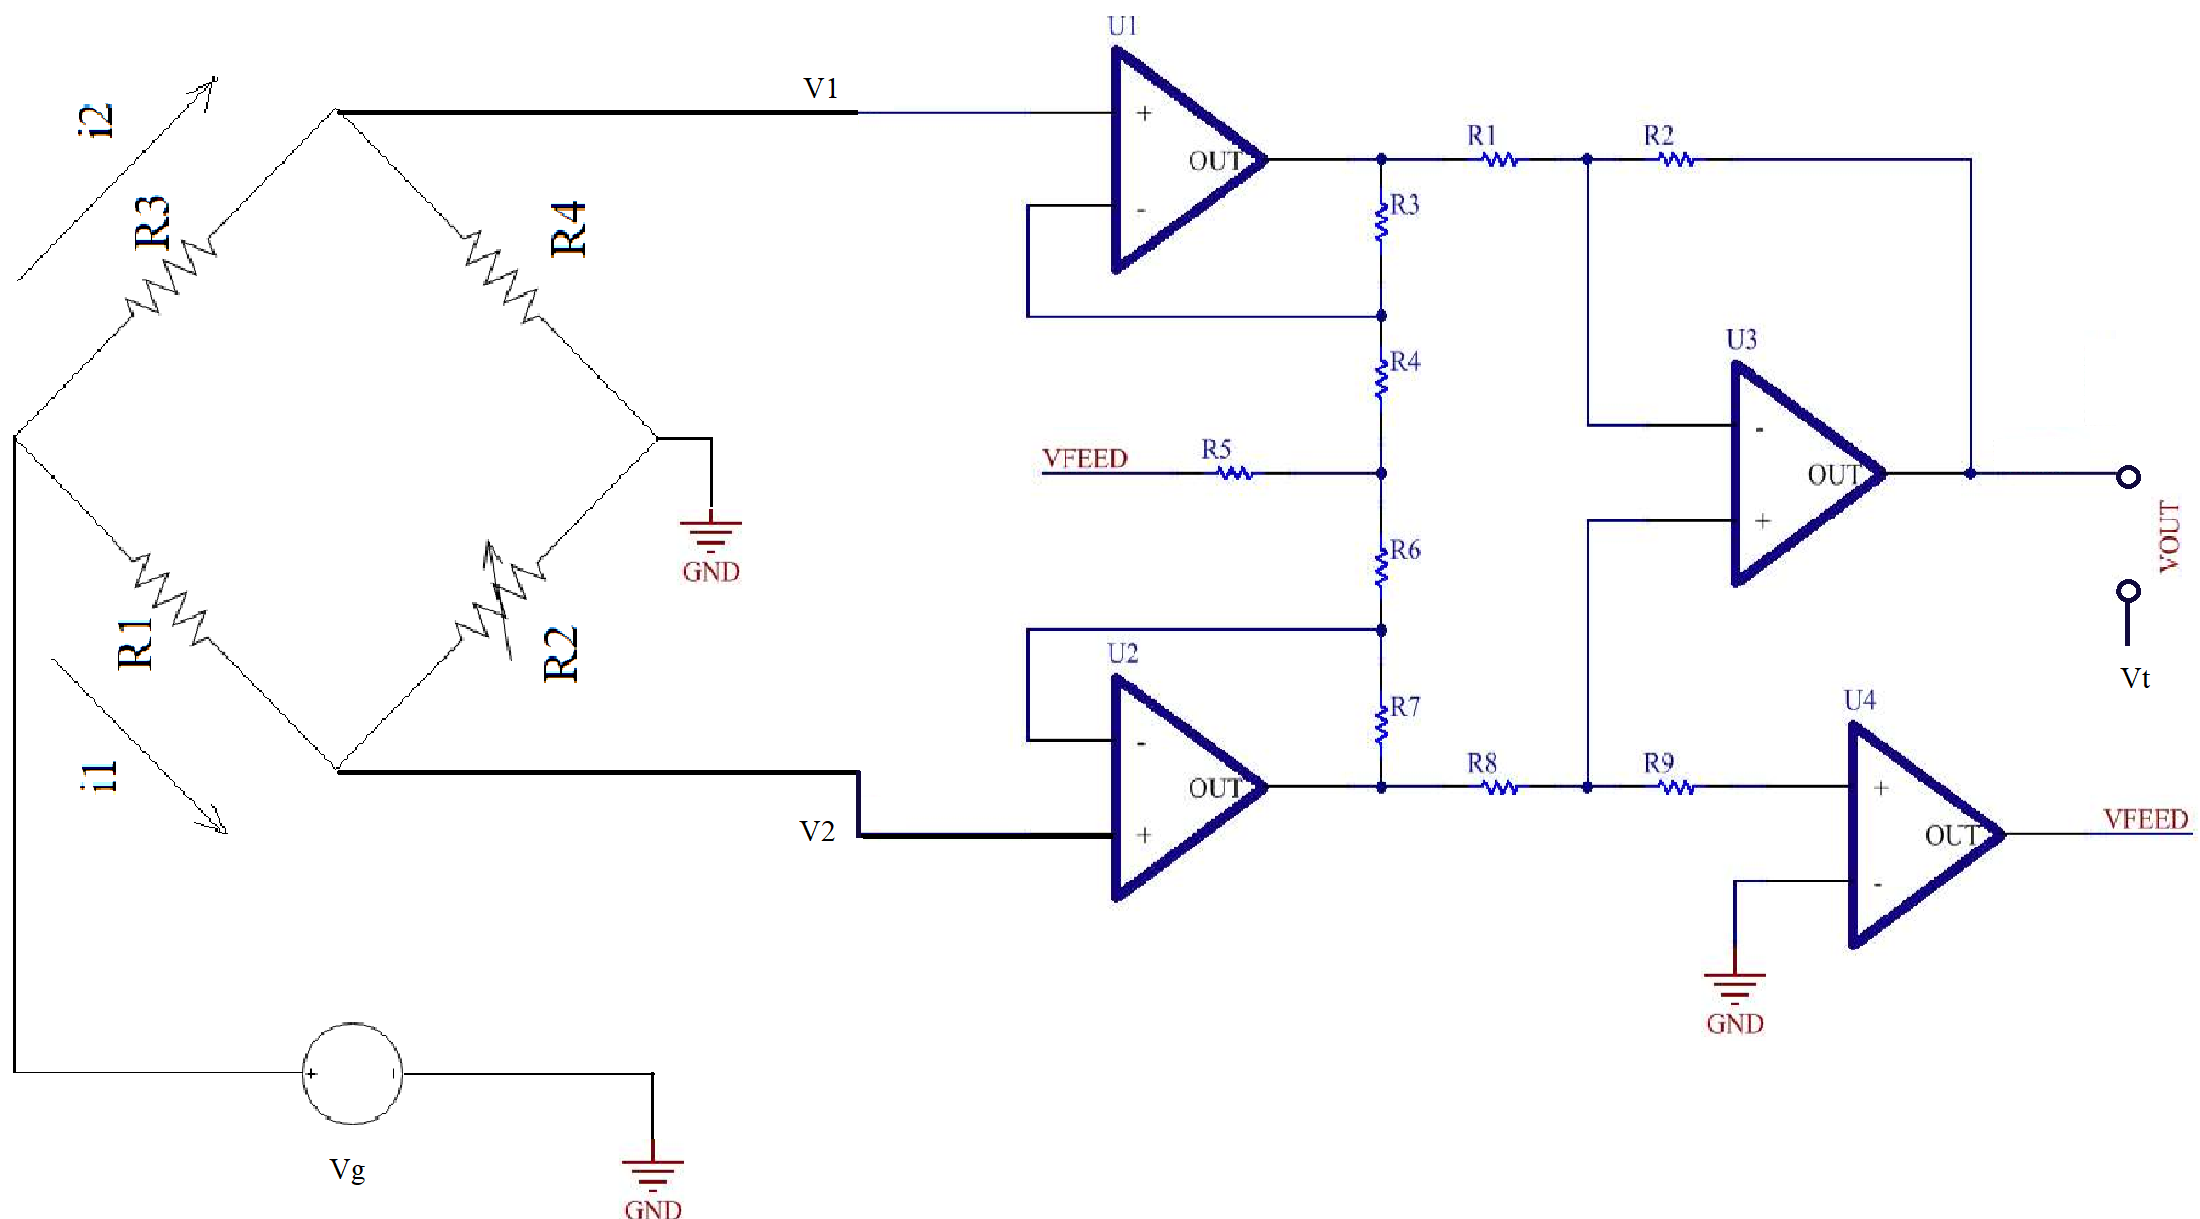
\includegraphics[scale=0.3]{imagenes/no_tierra_amp.png}
		\caption{Disposición del circuito con generador, tierra NO compartida.}
		\label{fig:ej5_no_tierra_amp}
	\end{figure}
	
%Simulaciones
\section{Simulaciones}
Las simulaciones fueron realizadas en LTSPICE.
%respuestas en frecuencia
	\begin{figure*}[h!]	
		\centering
		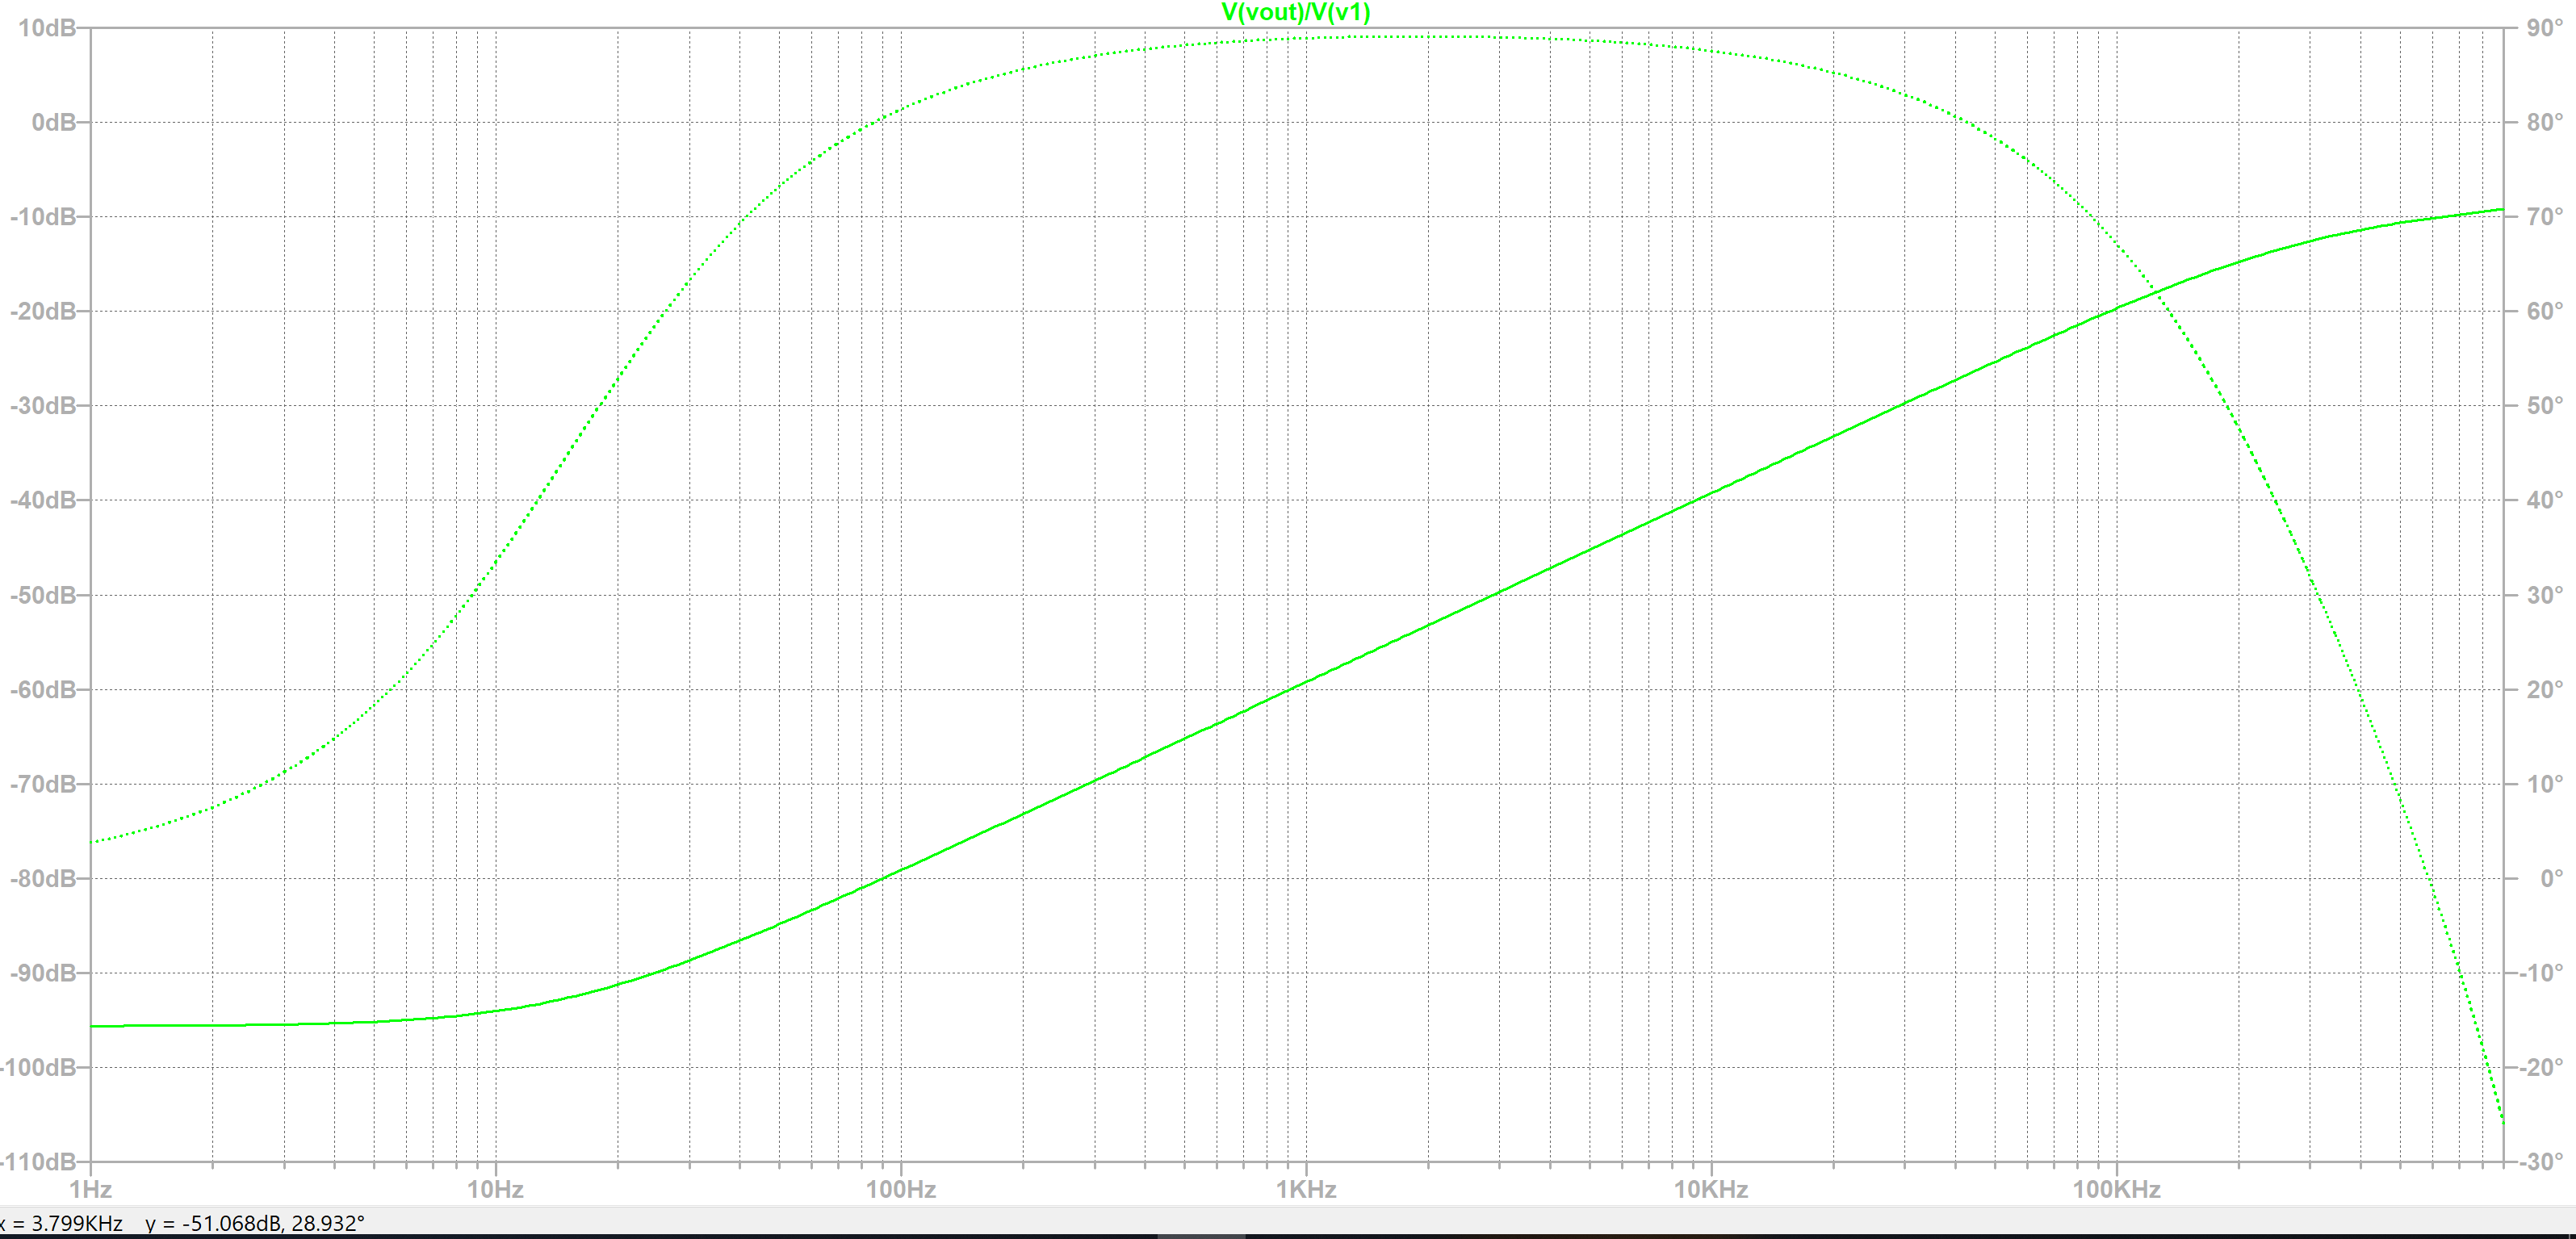
\includegraphics[scale=0.3]{imagenes/bode_comun_simulado.png}
		\caption{Respuesta en frecuencia simulada para el modo común}
		\label{fig:ej5_bode_diferencial_simulado}
	\end{figure*}

Debe tenerse en cuenta el error en el cálculo de ganancia comentado anteriormente!\par
Se muestra como el CMRR va disminuyendo exponencialmente (linealmente en escala logarítmica) a medida que se aumenta la frecuencia. Esto se debe a que la atenuación del modo común disminuye mientras que la amplificación del modo diferencial se mantiene práticamente constante en el mismo rango de frencuencias.\par

	\begin{figure*}[h!]	
		\centering
		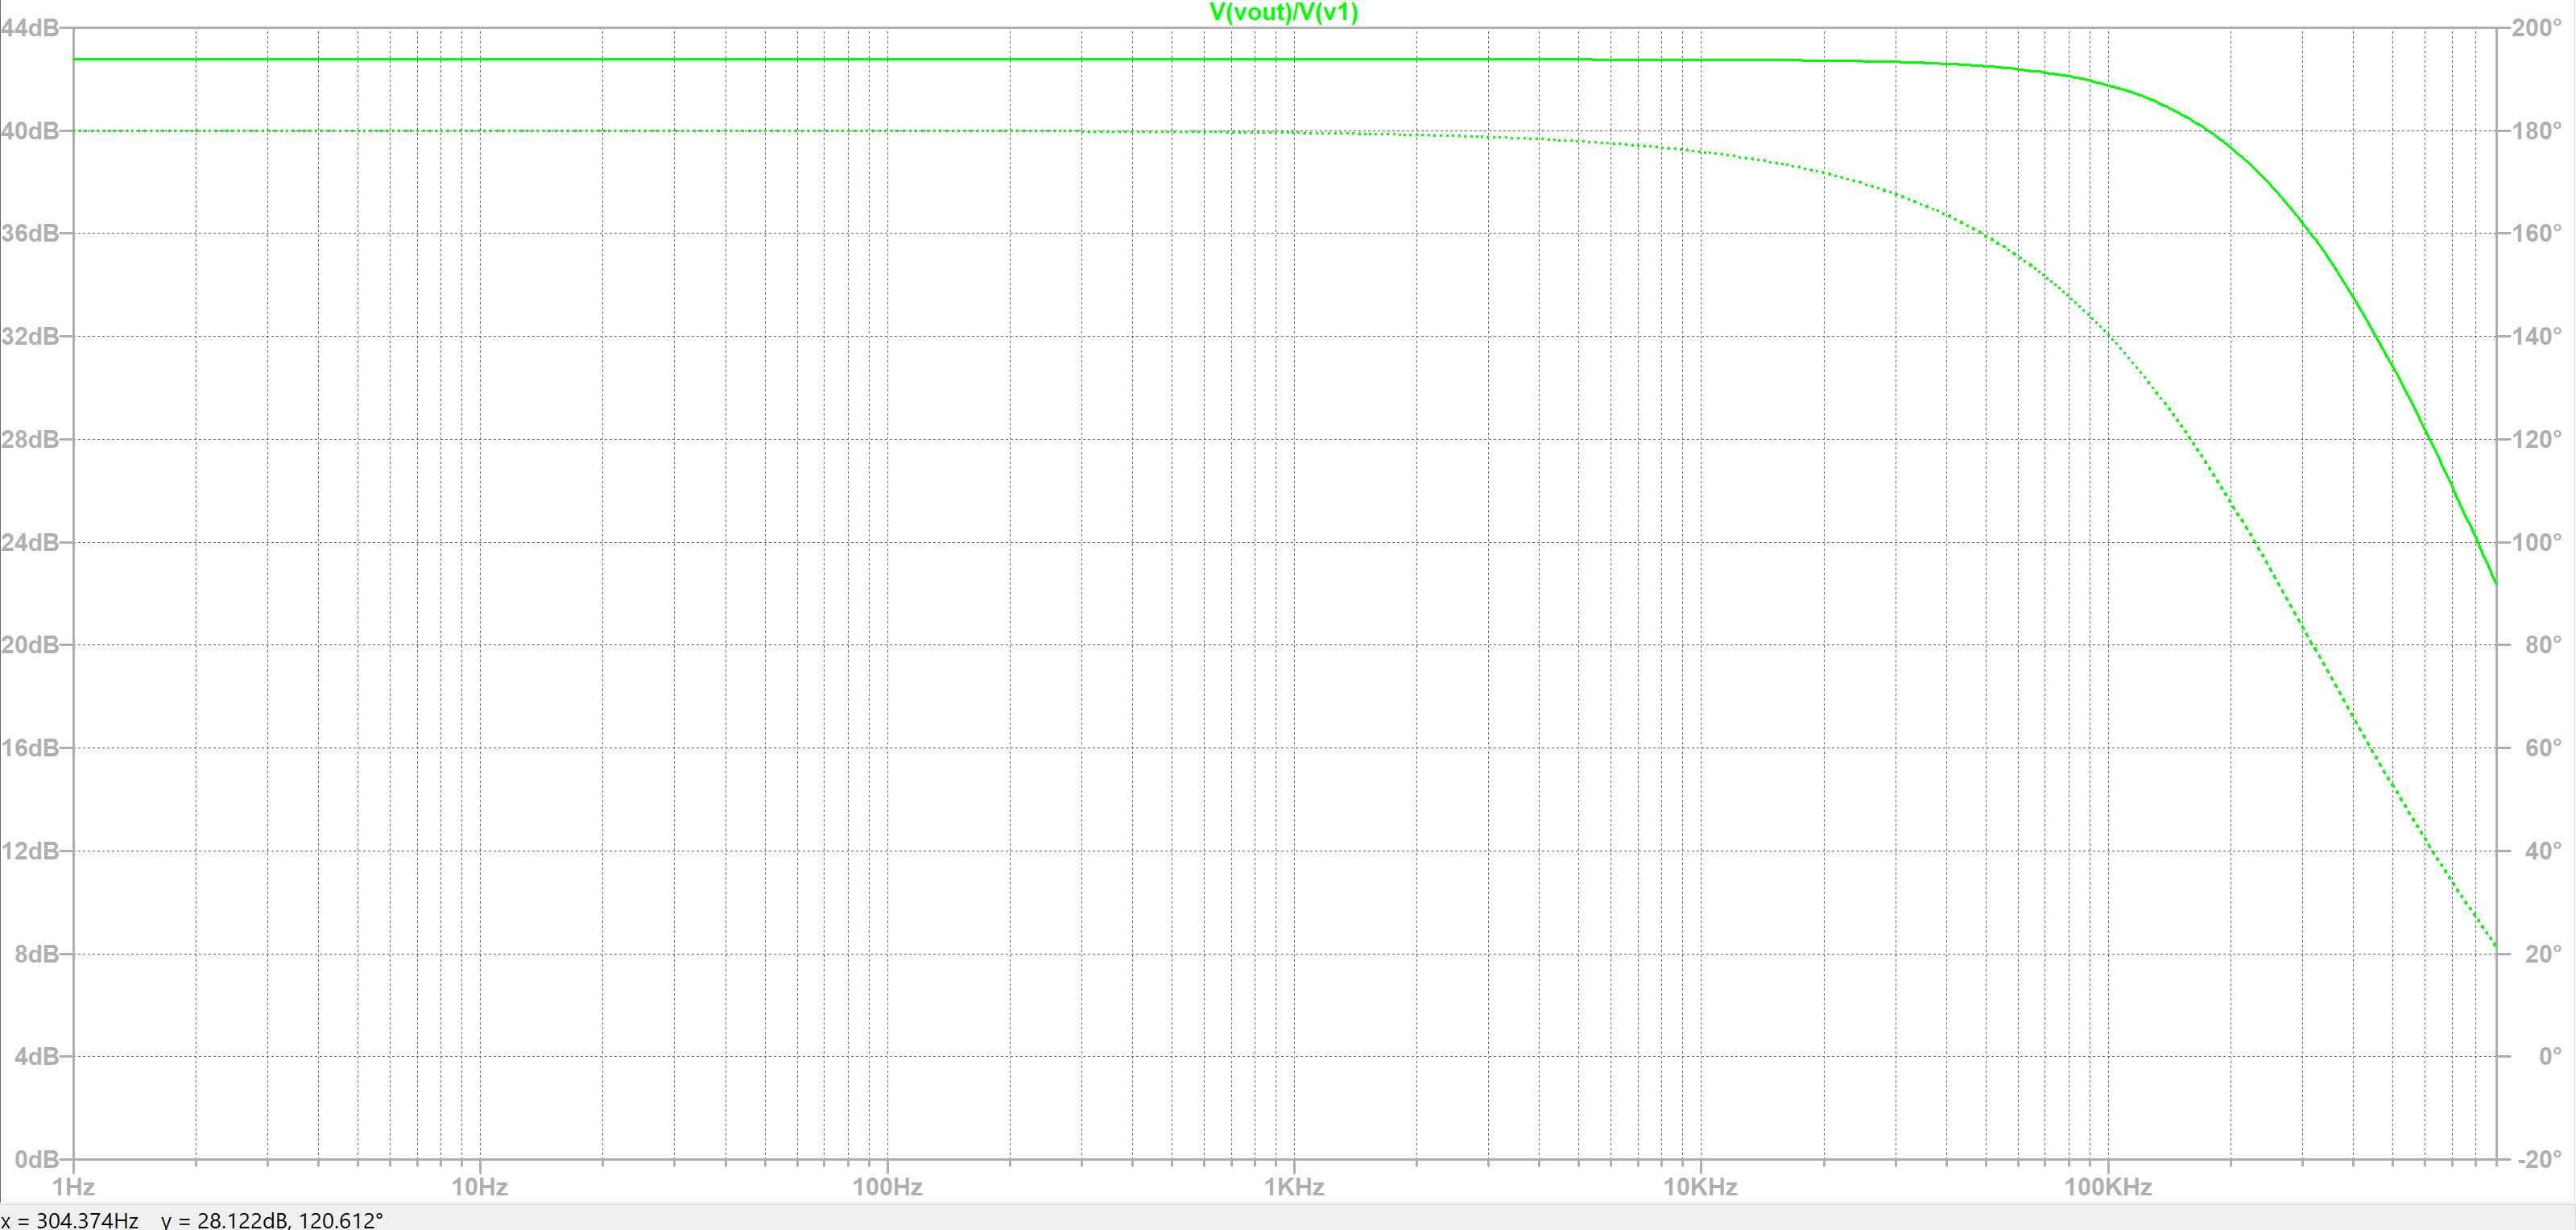
\includegraphics[scale=0.3]{imagenes/bode_diferencial_simulado.png}
		\caption{Respuesta en frecuencia simulada para el modo diferencial}
		\label{fig:ej5_bode_diferencial_simulado}
	\end{figure*}
	
	Se observa de la imagen anterior como la ganancia de
%muestra entrada salida	
	\begin{figure*}[h!]	
		\centering
		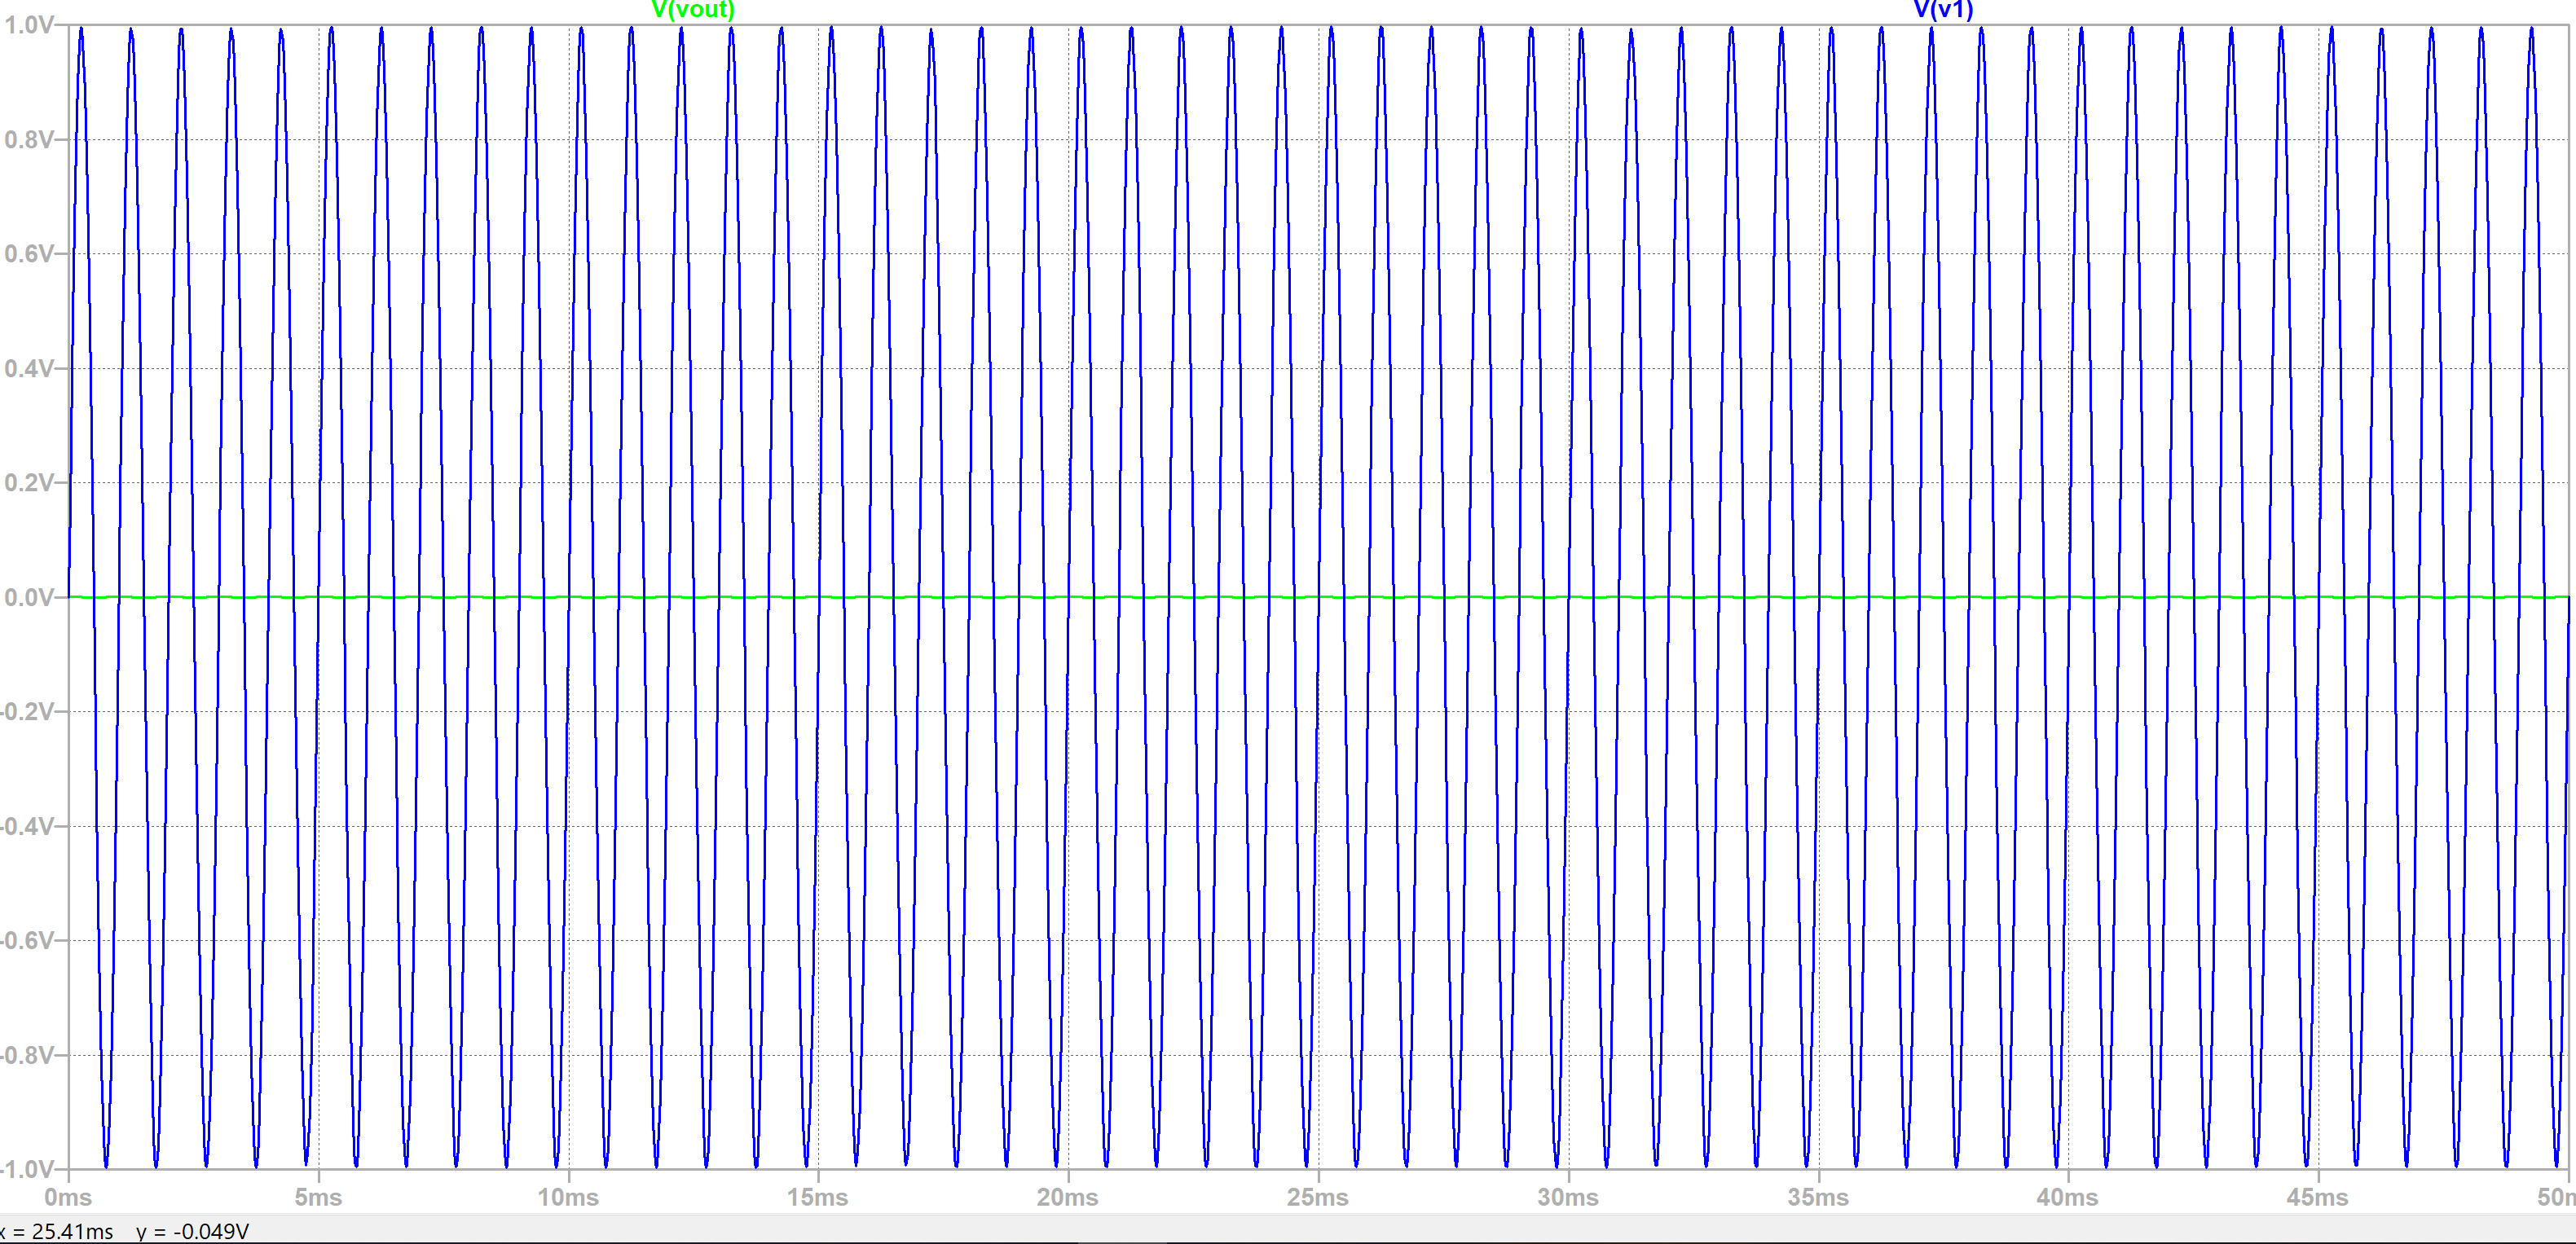
\includegraphics[scale=0.4]{imagenes/ganancia_comun_simulado.png}
		\caption{Simulación de la entrada y salida en modo común a 1kHz}
		\label{fig:ej3_ganancia_comun_simulado}
	\end{figure*}
	
	\begin{figure*}[h!]	
		\centering
		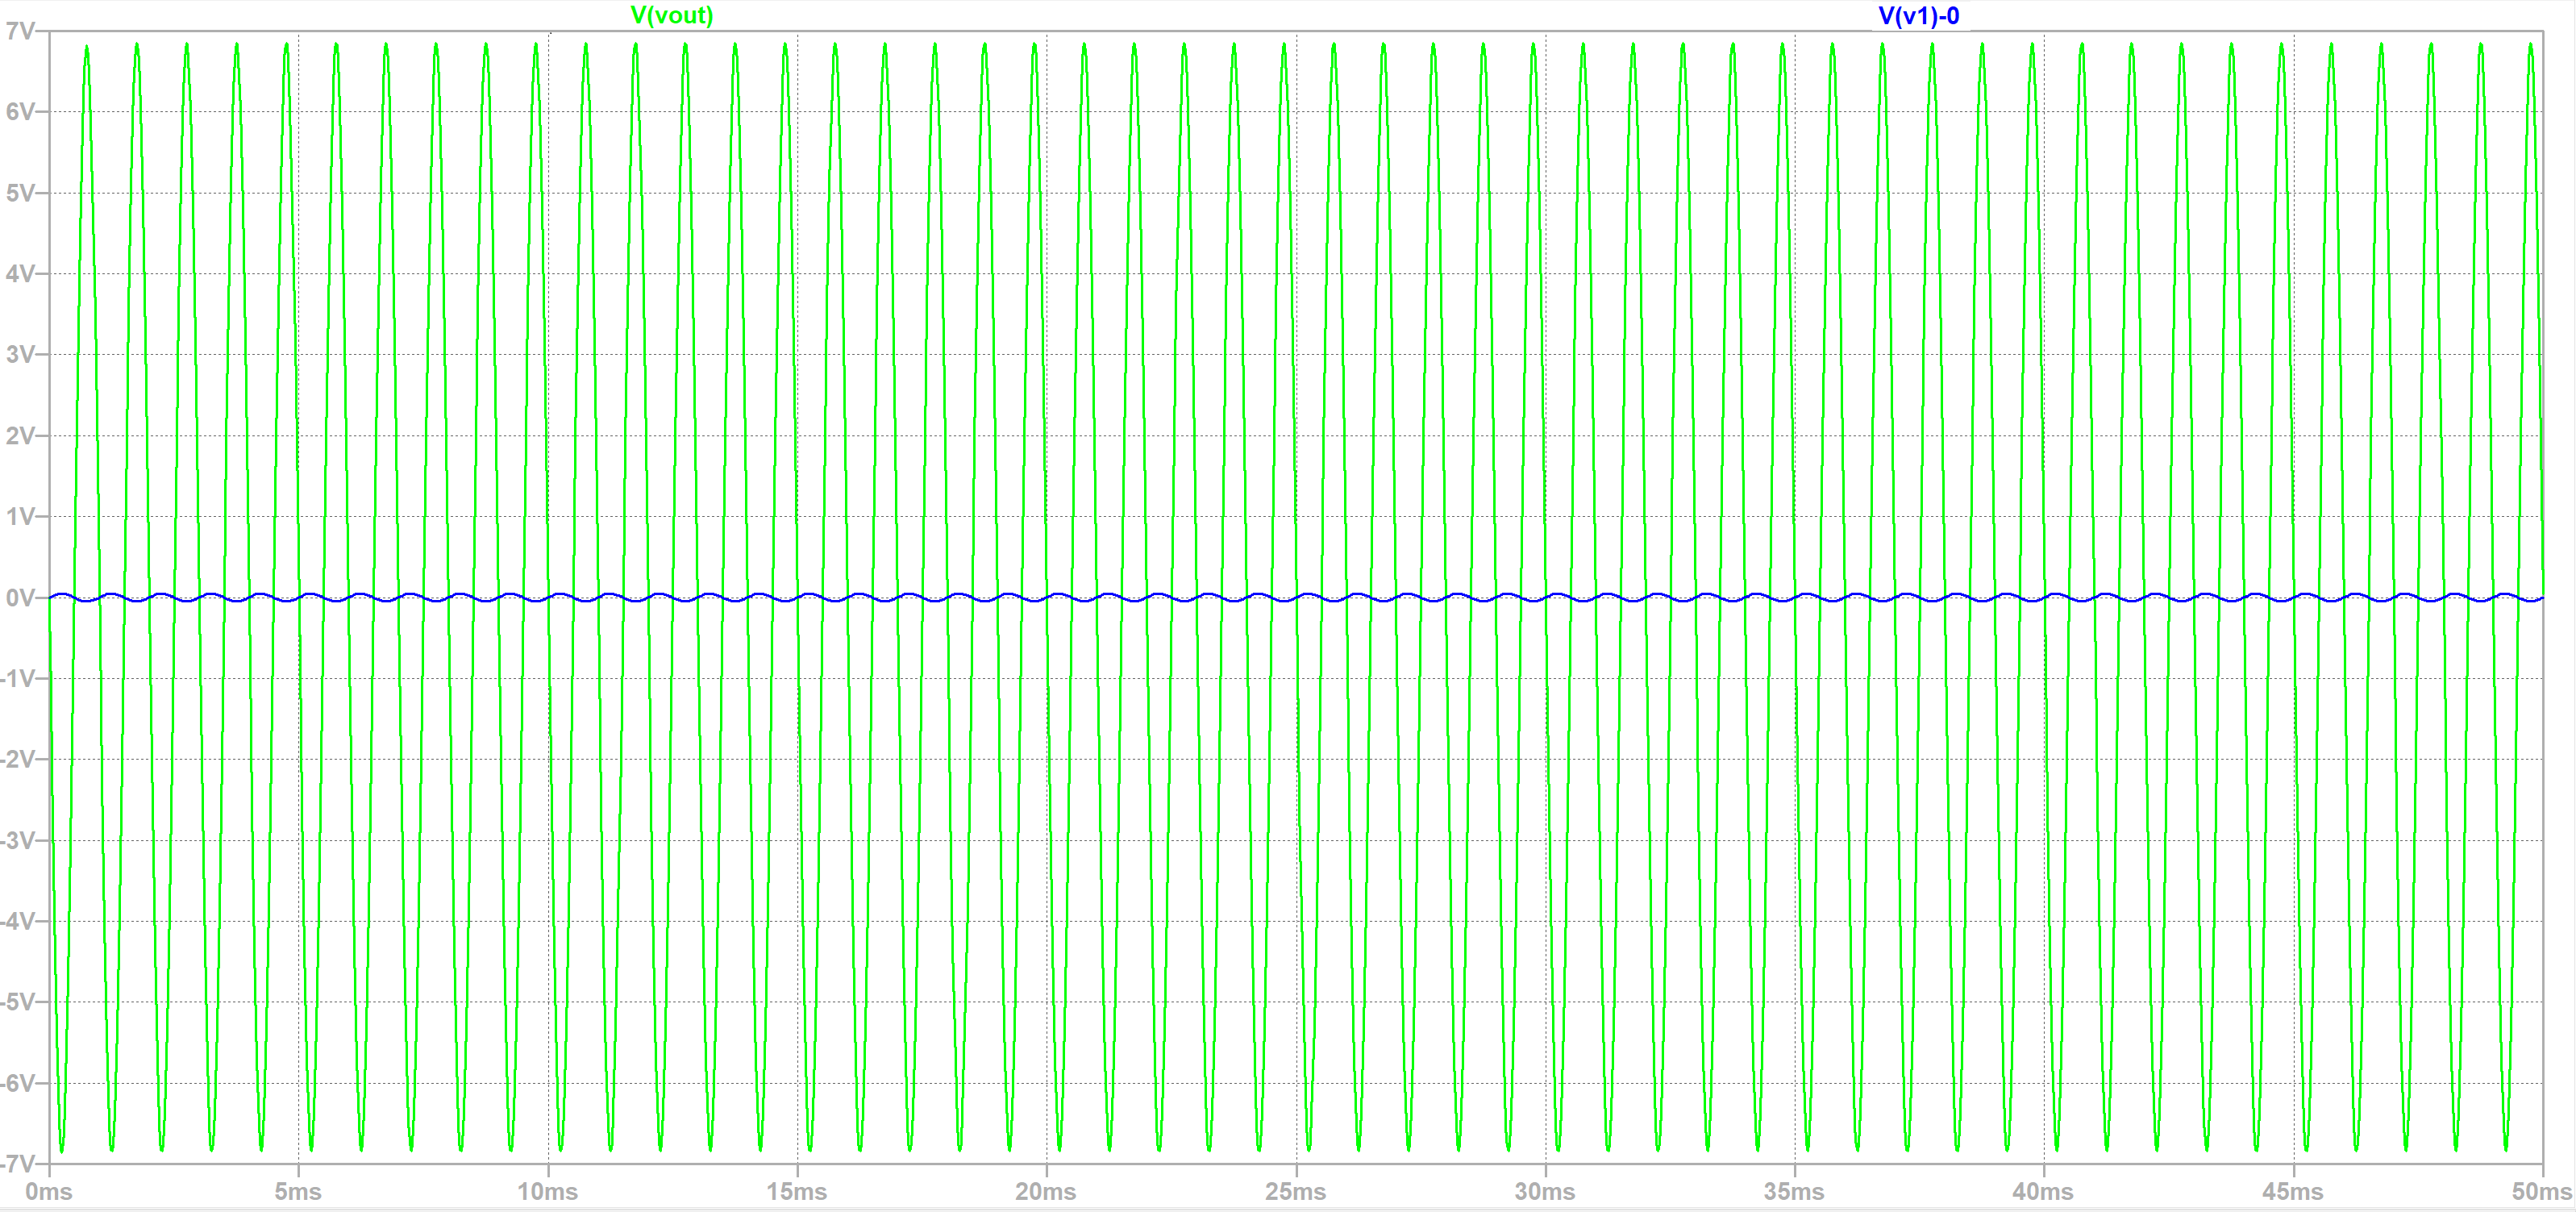
\includegraphics[scale=0.4]{imagenes/ganancia_diferencial_simulado.png}
		\caption{Simulación de la entrada y salida en modo diferencial a 1kHz}
		\label{fig:ej3_ganancia_diferencial_simulado}
	\end{figure*}
	
%Mediciones
\section{Mediciones}

Encontrará las imágenes de las simulaciones y las mediciones al final del ejercicio.\par

Las mediciones se realizaron con un analog discovery 2.\par
Las ondas de baja amplitud fueron generadas mediante el uso del puente de Wheatstone conectado de la manera explicada en la sección anterior.
Para la respuesta en frecuencia, se comenzó a medir a partir de 1kHz porque el modo común estaba demasiado atenuado para frecuencias menores a ese valor como para ser medido. \par
Esta respuesta en frecuencia nos dará la ganancia del modo común a partir de la cual se consigue el CMRR.

%respuestas en frecuencia
		\begin{figure*}[h!]	
		\centering
		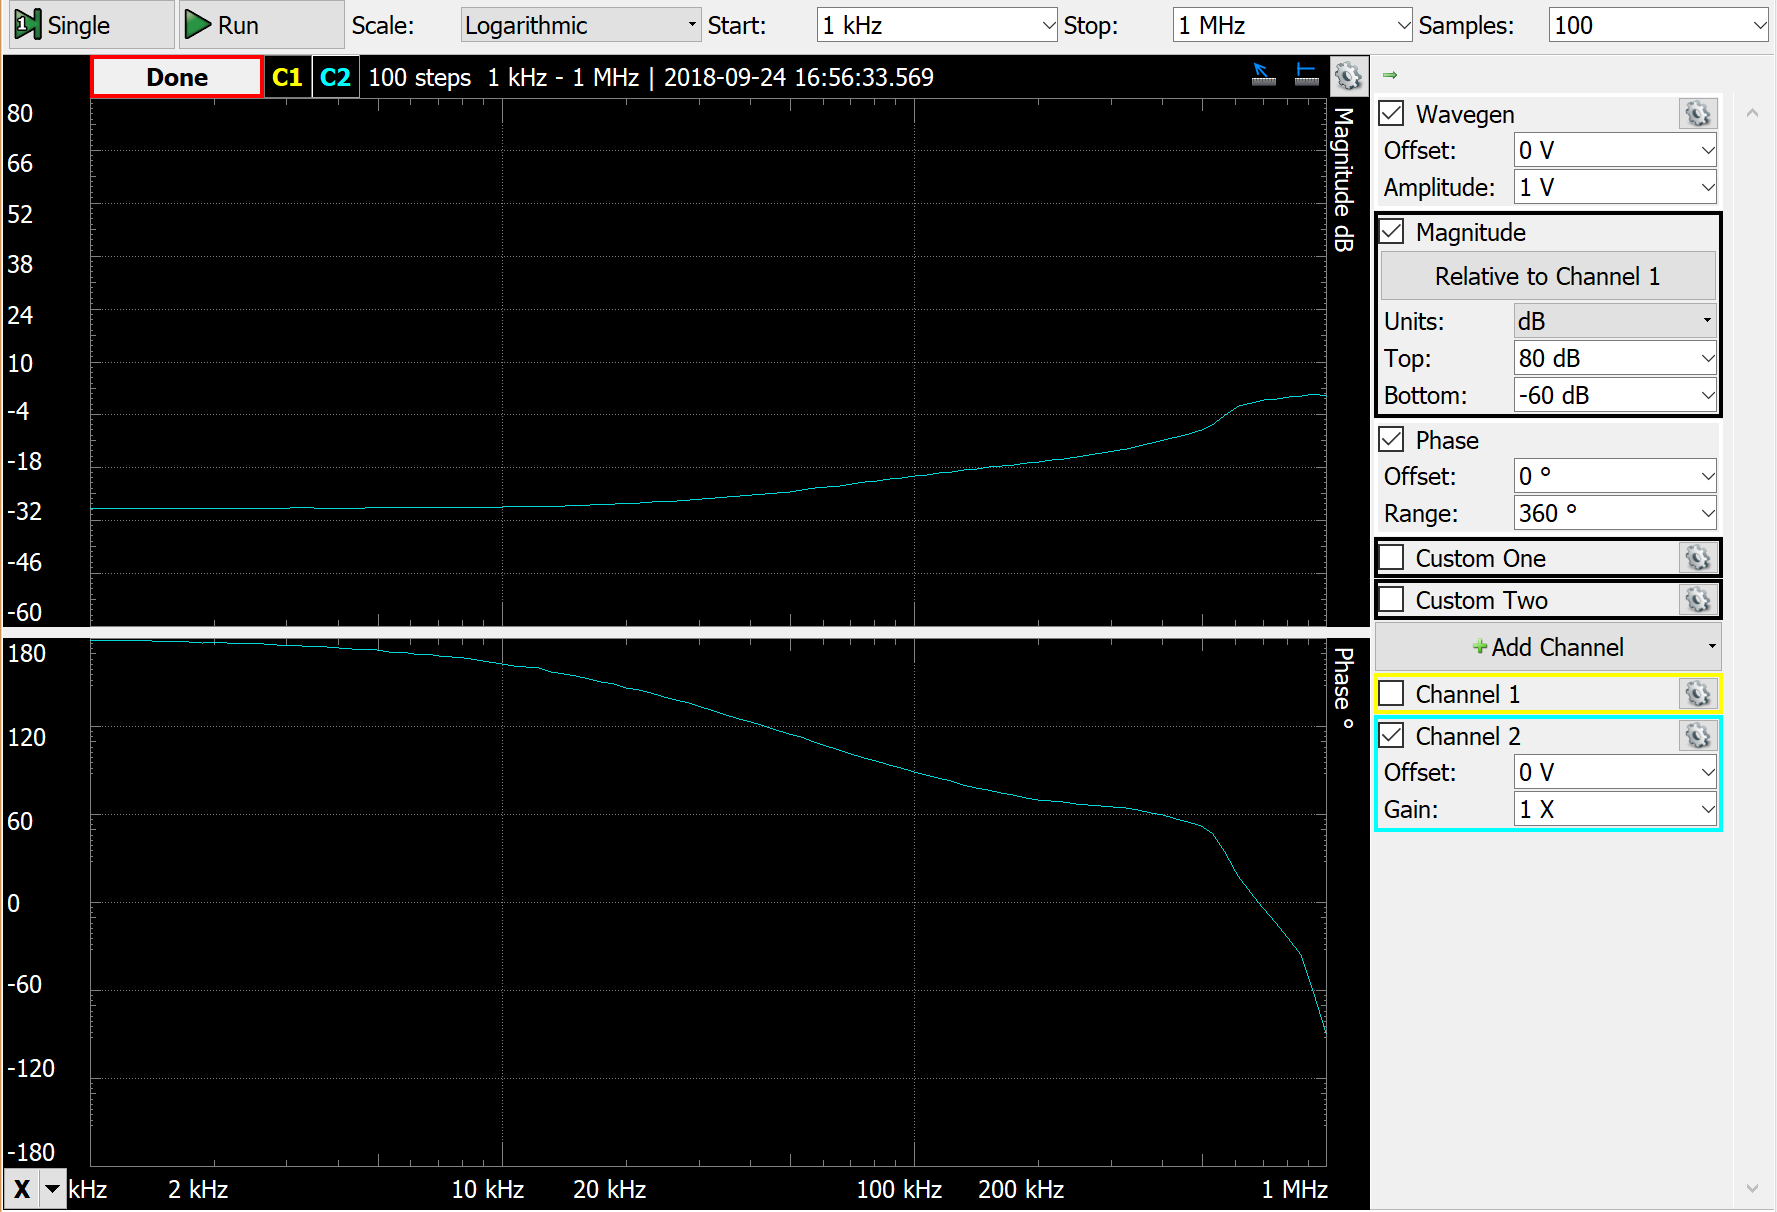
\includegraphics[scale=0.6]{imagenes/bode_comun_medido.png}
		\caption{Respuesta en frecuencia medida para el modo común}
		\label{fig:ej3_bode_comun_medido}
	\end{figure*}
	La menor atenuación del modo común medido contra el teórico se cree que se debe a la presencia de armónicos provenientes de una fuente no ideal, además de la imposibilidad de medir a partir de cierta atenuación por parte del osciloscopio para una entrada de 1 V de amplitud, que en futuros trabajos se elevará en magnitud en caso de deber medir atenuaciones tan grandes.\par
	Se observa la misma forma para la respuesta en frecuencia de la curva simulada con la medida: mismos puntos de inflexión, zonas lineales y zonas planas en los mismos rangos de frecuencia.\par
	En cuanto a la fase,  si bien se puede apreciar la forma de campana de la simulación, se encuentra que la fase comienza a sufrir cambios contra lo esperado para frecuencias mayores a 100k. \par
	Dado el análisis anterior, se espera que el circuito funcione correctamente para frecuencias de hasta 100kHz.
	El siguiente análisis de montecarlo muestra claramente que la respuesta en frecuencia lograda estaba dentro de lo esperado:
	
			\begin{figure*}[h!]	
		\centering
		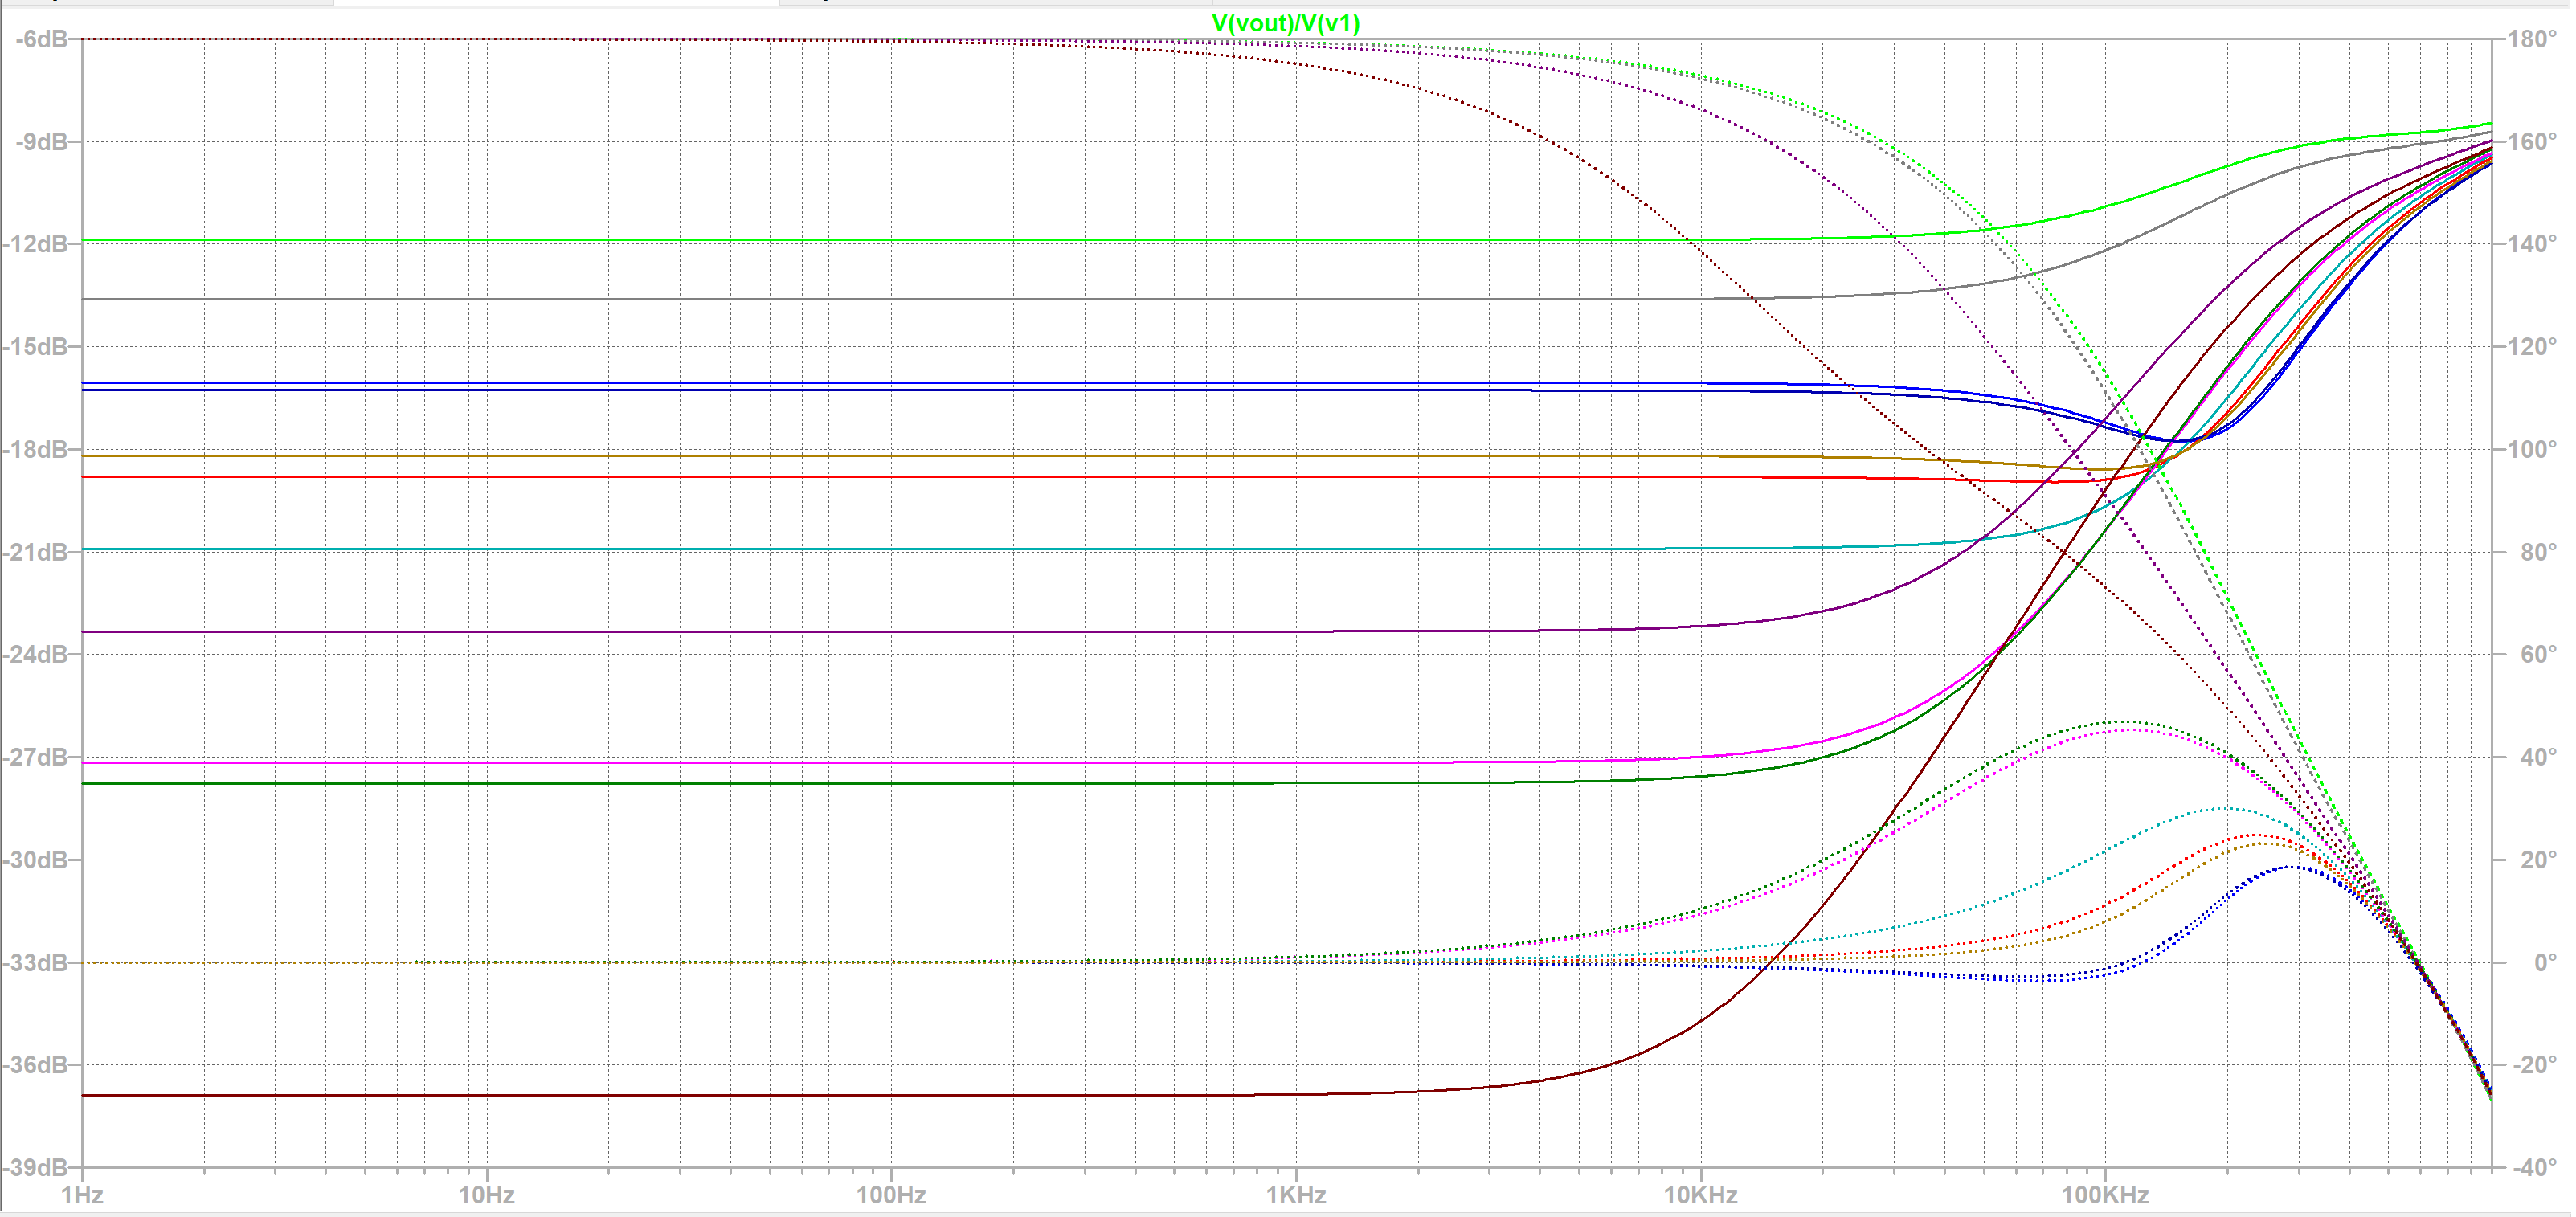
\includegraphics[scale=0.4]{imagenes/bode_comun_montecarlo.png}
		\caption{Análisis de montecarlo}
		\label{fig:ej3_bode_comun_medido}
	\end{figure*}
	
	Se muestra de aquí que el sistema es altamente sensible a las tolerancias. Sin embargo, la razón de ser el opamp U4 es lograr calibrar el sistema en tiempo real de modo tal que no se tenga que usar presets para su calibración al contar con resistencias no ideales (las relaciones no se cumplen estrictamente), por lo que es predecible que esta calibración o mejora en precisión se pague con una menor atenuación del modo común y una peor ganancia para el modo diferencial.
	%muestra entrada salida
			\begin{figure*}[h!]	
		\centering
		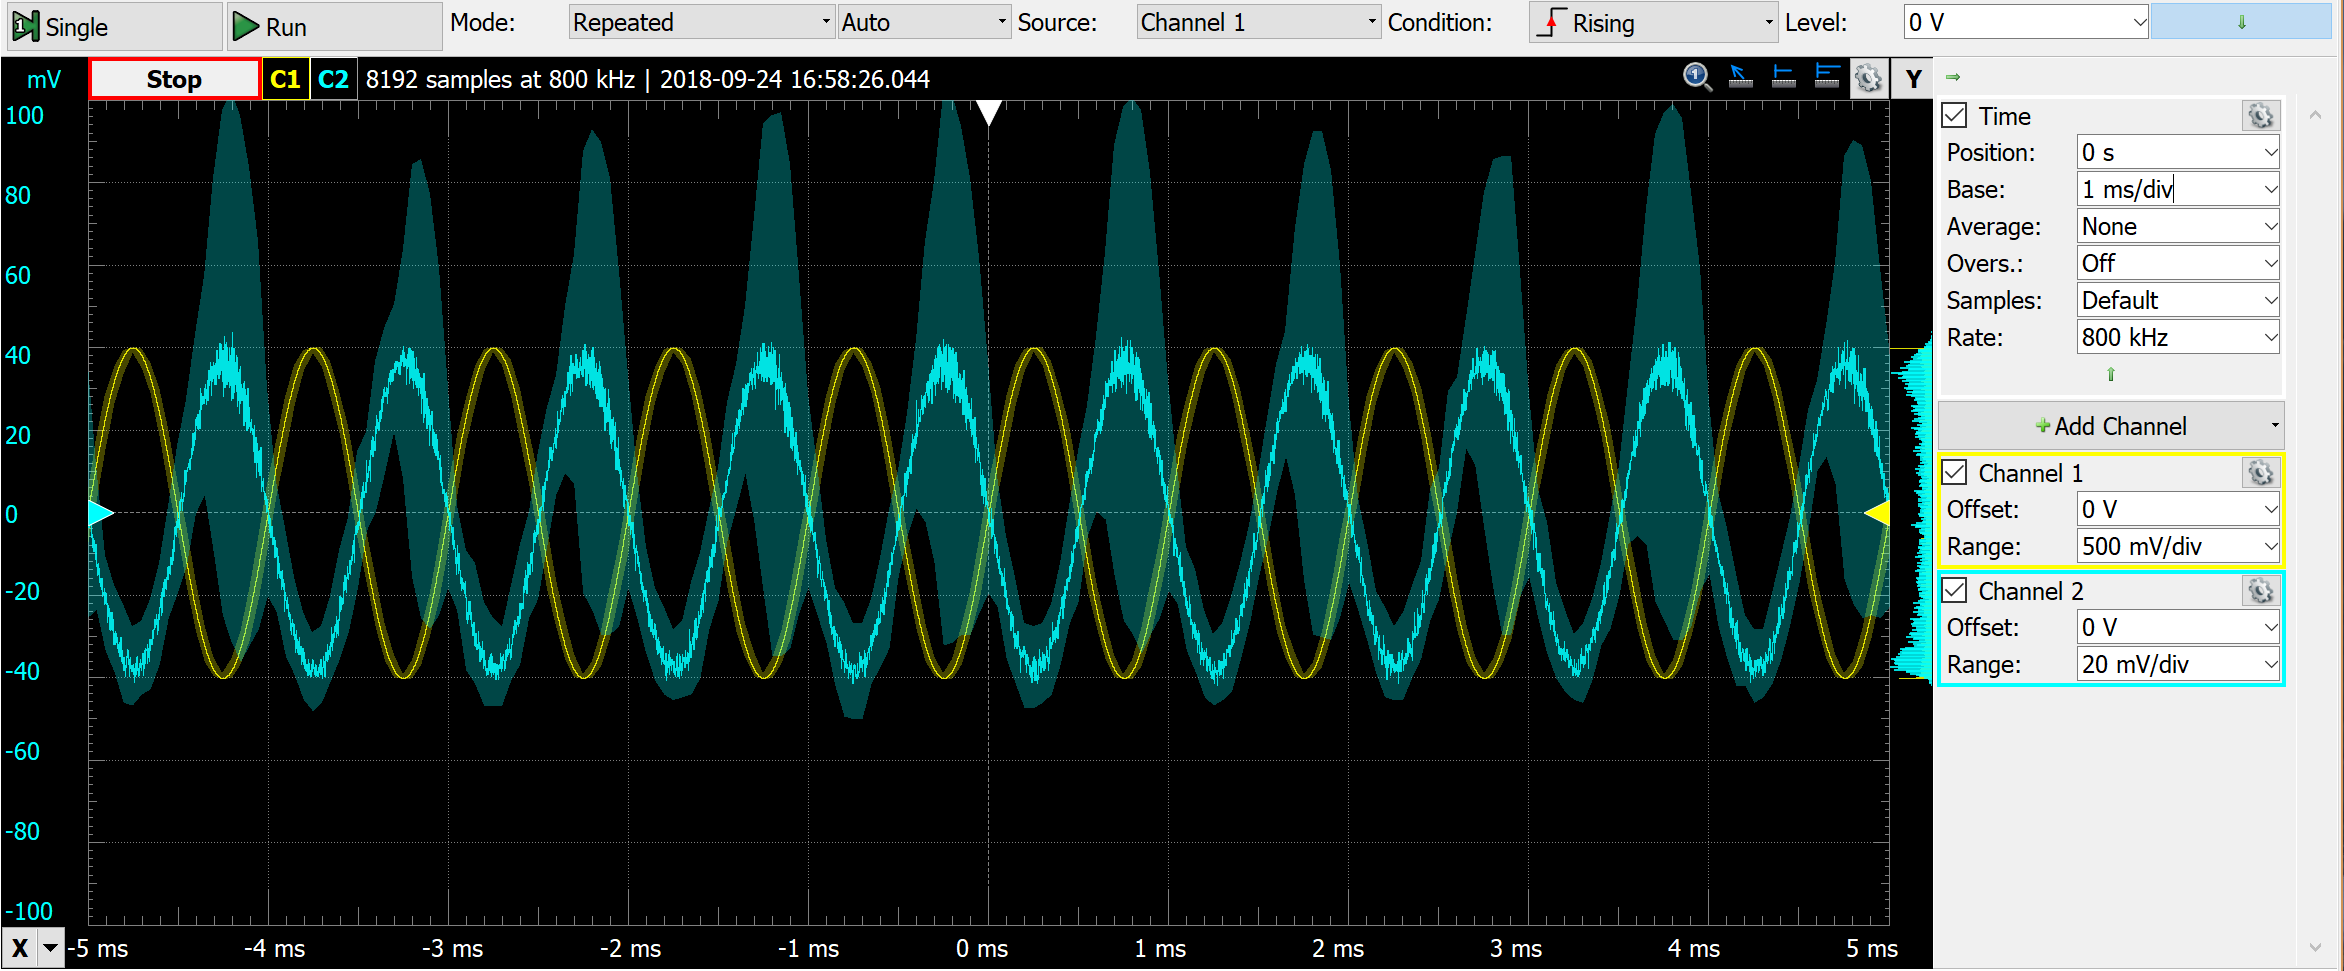
\includegraphics[scale=0.6]{imagenes/ganancia_comun_medido.png}
		\caption{Muestra de la entrada y salida en modo común a 1kHz}
		\label{fig:ej3_ganancia_comun_medido}
	\end{figure*}
	
	A continuación se presentan el gráfico de bode en modo diferencial.
	
	\begin{figure*}[h!]	
		\centering
		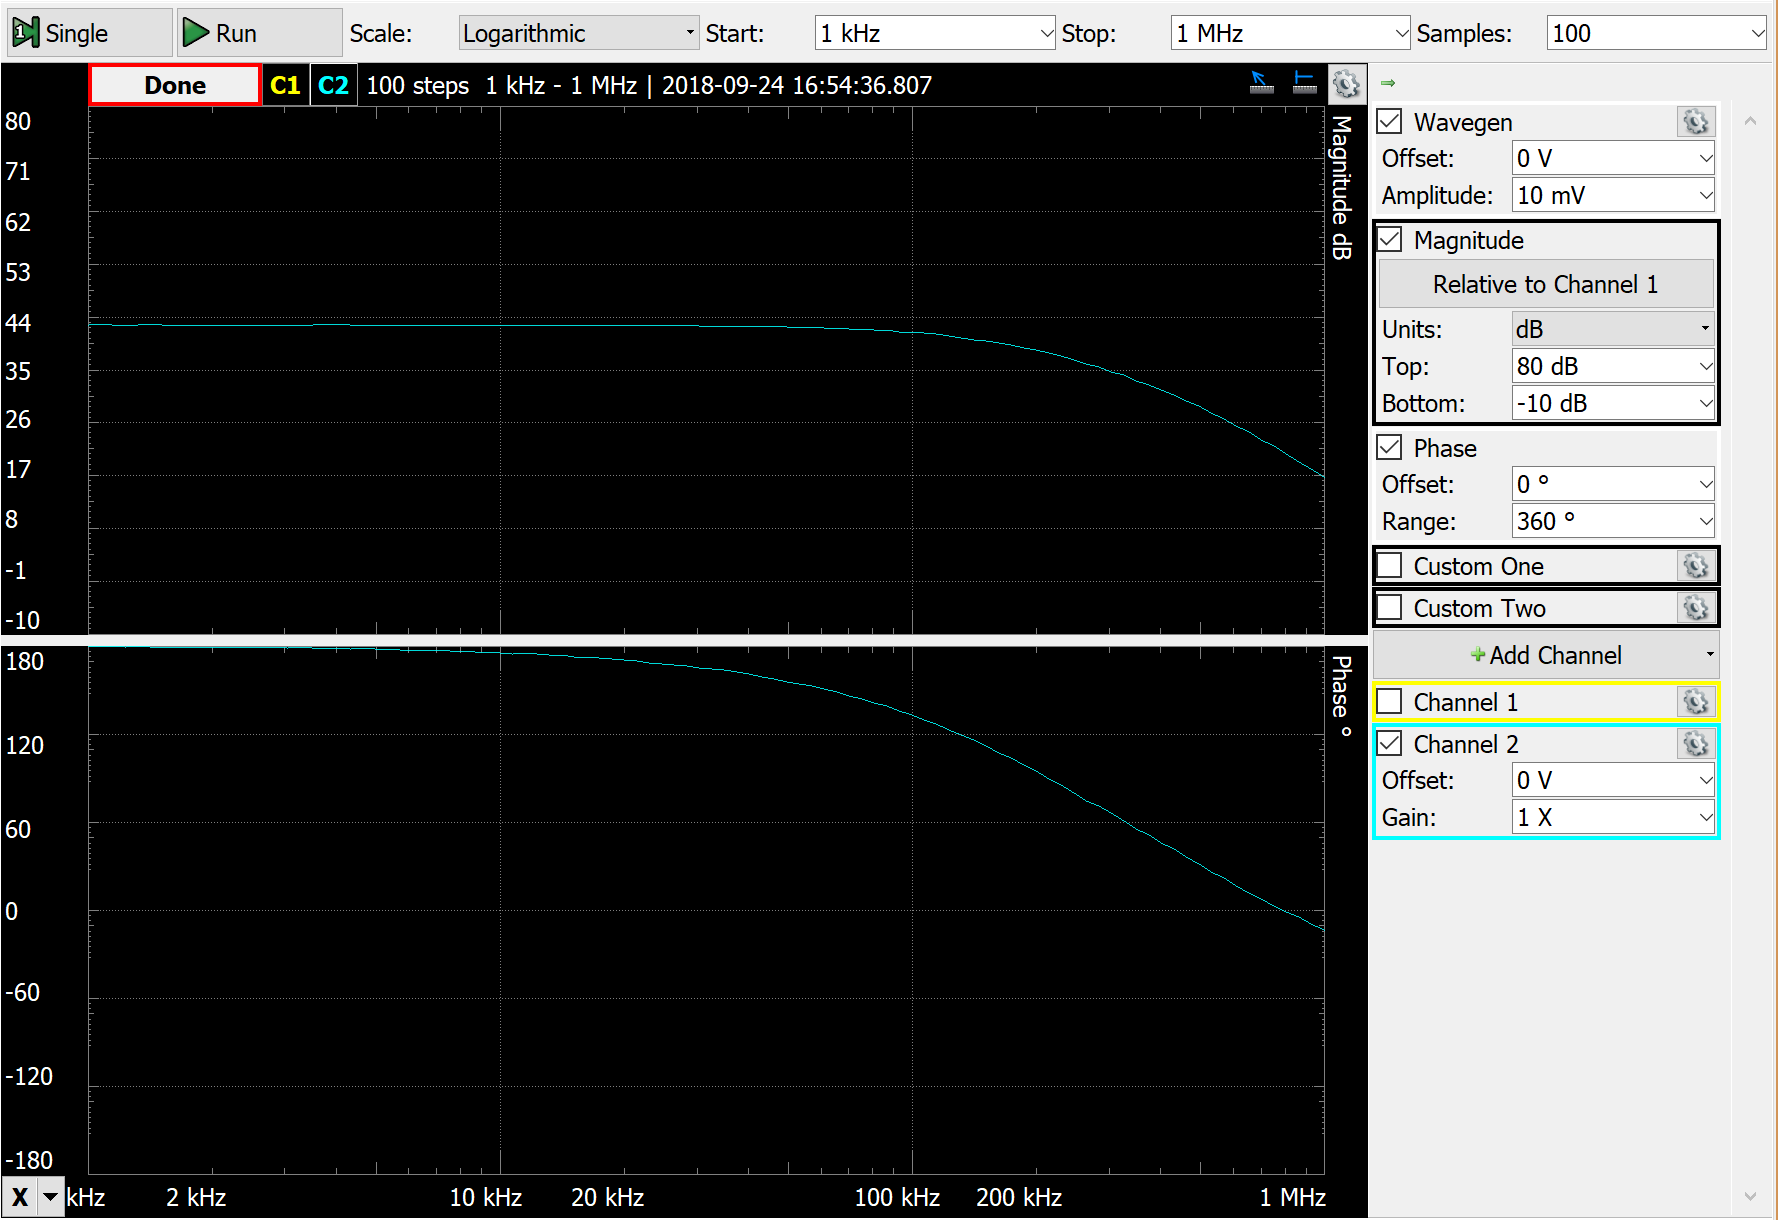
\includegraphics[scale=0.6]{imagenes/bode_diferencial_medido.png}
		\caption{Respuesta en frecuencia medida para el modo diferencial}
		\label{fig:ej3_bode_diferencial_medido}
	\end{figure*}
	Se corrobora lo medido como lo simulado en módulo y fase, por lo que un análisis de montecarlo parece innecesario.
	
		\begin{figure*}[h!]	
		\centering
		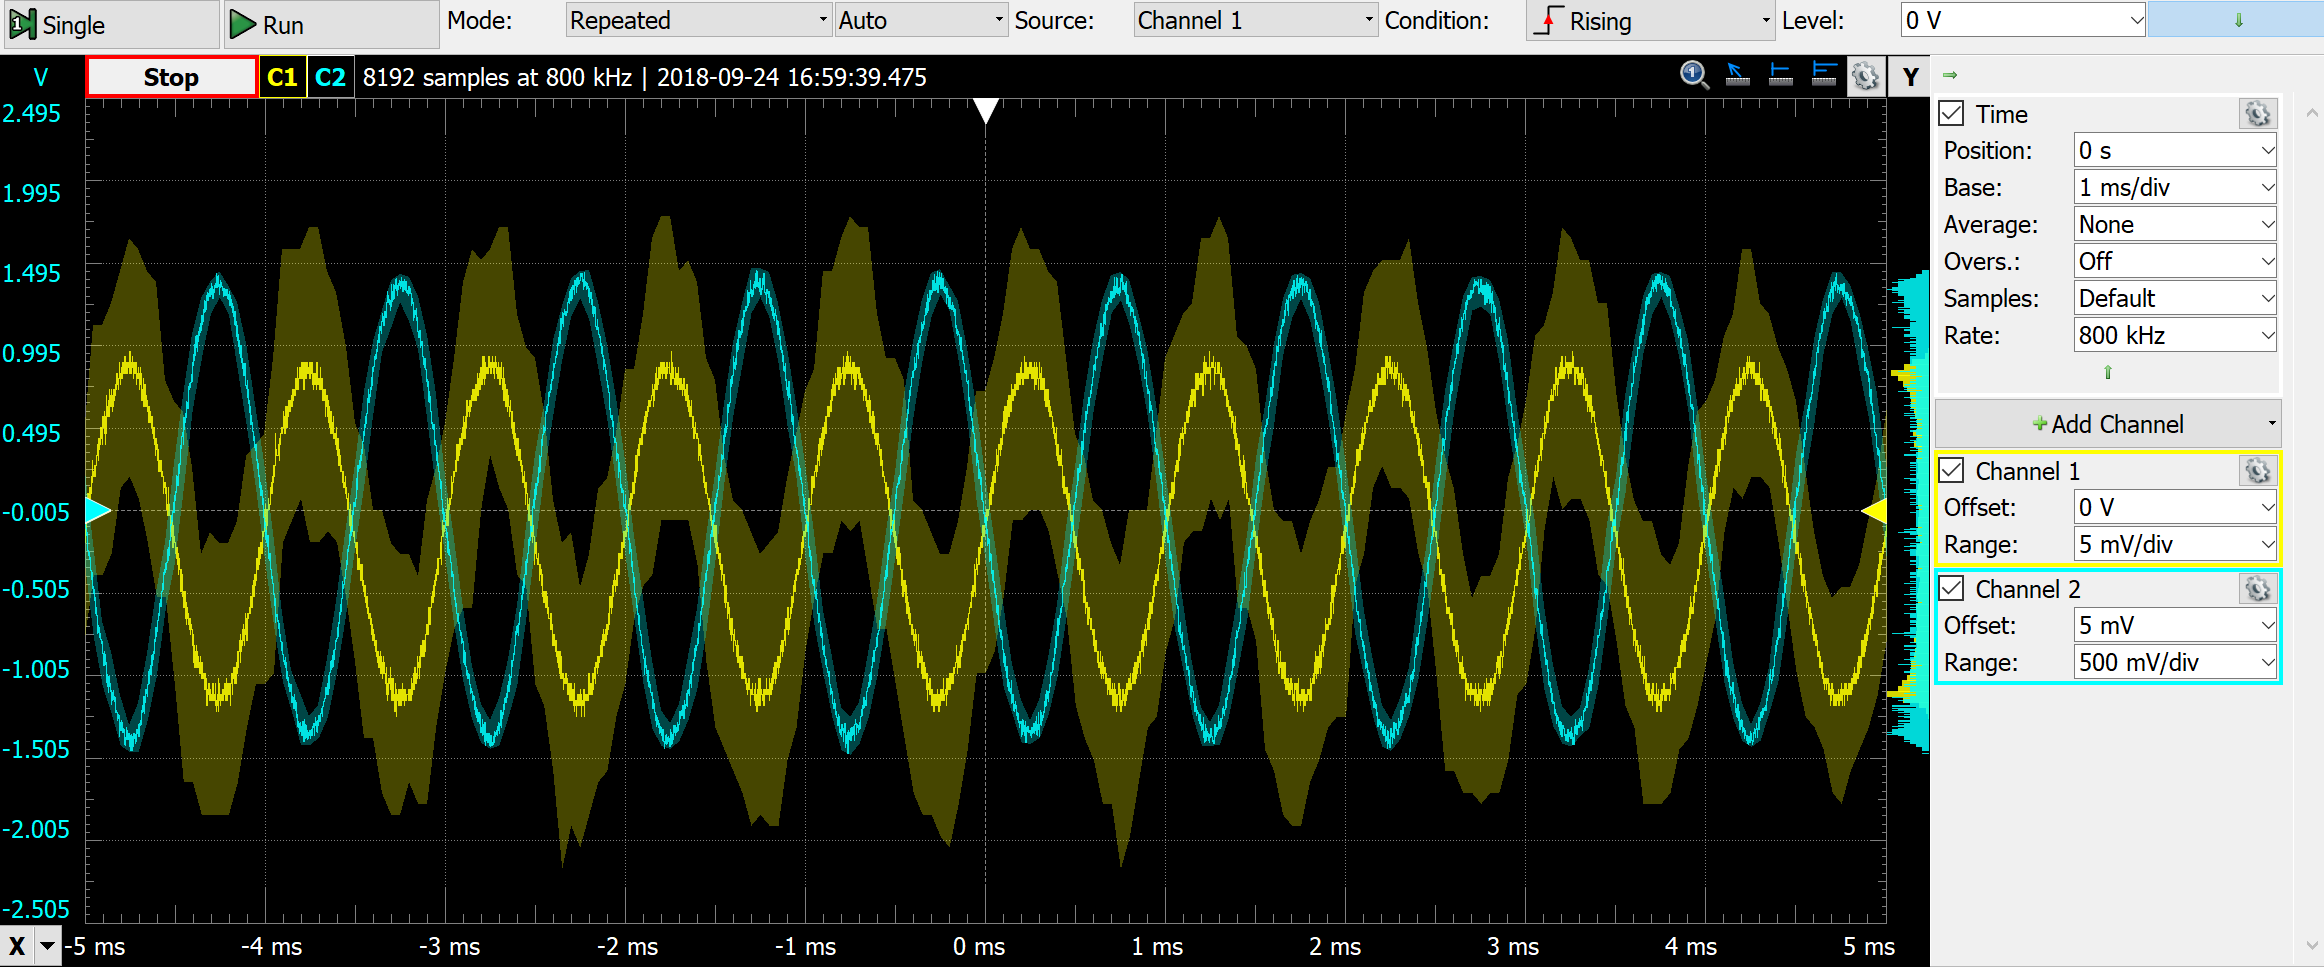
\includegraphics[scale=0.6]{imagenes/ganancia_diferencial_medido.png}
		\caption{Muestra de la entrada y salida en modo diferencial a 1kHz}
		\label{fig:ej3_ganancia_diferencial_medido}
	\end{figure*}

		\begin{figure*}[h!]	
		\centering
		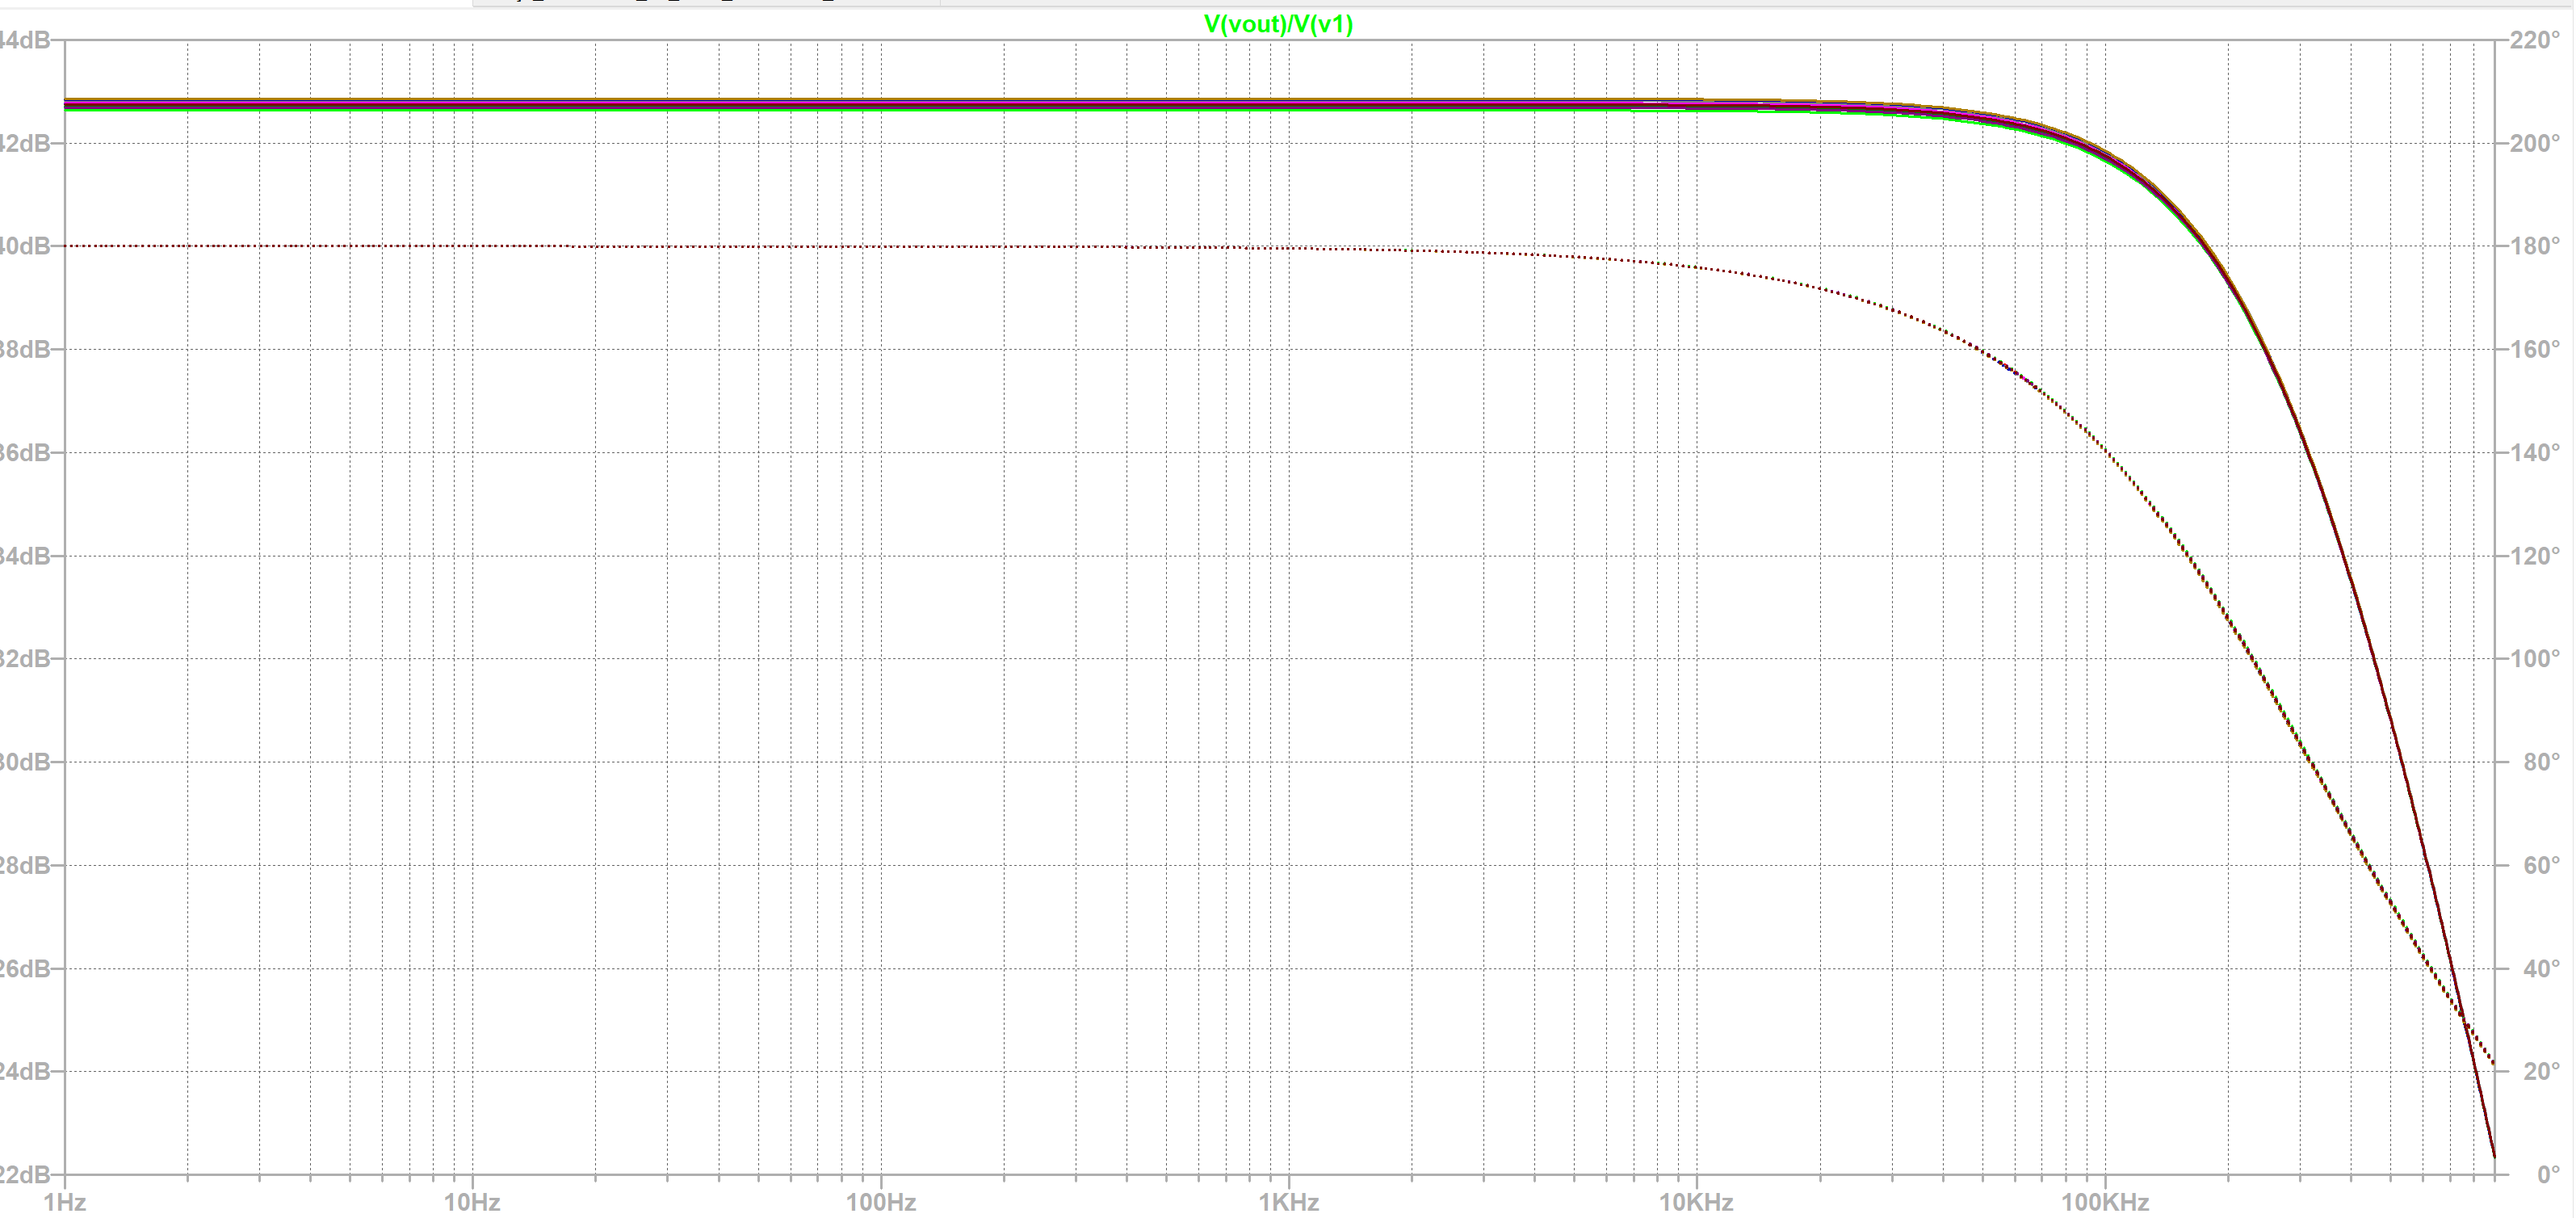
\includegraphics[scale=0.4]{imagenes/bode_diferencial_montecarlo.png}
		\caption{Bode diferencial, análisis de montecarlo}
		\label{fig:ej3_bode_diferencial_montecarlo}
	\end{figure*}

\section{Conclusión}

Se logró implementar exitosamente el amplificador instrumental, utilizando un generador de señales de baja amplitud realizado mediante el uso de un puente de Wheatstone.


\clearpage\newpage


\end{document}
